\PassOptionsToPackage{quiet}{fontspec} % 抑制中文字体警告
\documentclass[12pt,AutoFakeSlant,AutoFakeBold]{article}
\usepackage{ctex}
\usepackage[a4paper,top=2.5cm,bottom=2.5cm,left=2.5cm,right=2.5cm]{geometry}

% Useful packages
\usepackage{amsmath}
\usepackage{graphicx}
\usepackage[colorlinks=true, allcolors=blue]{hyperref}
\usepackage{booktabs}
\usepackage{subfigure}
\usepackage{enumitem}
\usepackage{minted}
\usepackage{multirow}
\usepackage{titlesec}
\usepackage{amsfonts,amssymb}
\usepackage{minted}
\usepackage{longtable}
\usepackage{gbt7714}
\usepackage{mdwlist}
\usepackage[section]{placeins}
\usepackage{svg}
\titleformat*{\section}{\Large\centering}

\title{无人机遂行编队飞行中的纯方位无源定位}
\makeatletter
\let\Mytitle\@title
\makeatother

\counterwithin{figure}{section} %图片按照章节编号
\counterwithin{table}{section} %图片按照章节编号
\counterwithin{equation}{section} %图片按照章节编号

\begin{document}

%%%%%%%%%%%%%%%%%%%%%%%%%%%%%%%%%%%%%%%%%%%%%%%%%%%%%%%%%%%%%%%%
%%%%%%%%%%%%%%%%%%%%%%%%%%%%%%%%%%%%%%%%%%%%%%%%%%%%%%%%%%%%%%%%
%                           摘要页开始                          %
%%%%%%%%%%%%%%%%%%%%%%%%%%%%%%%%%%%%%%%%%%%%%%%%%%%%%%%%%%%%%%%%
%%%%%%%%%%%%%%%%%%%%%%%%%%%%%%%%%%%%%%%%%%%%%%%%%%%%%%%%%%%%%%%%

%输出标题
\centerline{\Huge\heiti\textbf{\Mytitle}}

\vspace{1em} %设置空行

%输出摘要二字
\centerline{\Large\heiti\textbf{摘\quad 要}}

\vspace{1em} %设置空行

在现代无人机编队飞行任务中,为最大化隐蔽性和安全性,无人机群体需尽量减少向外界发射电磁波信号,以避免被敌方探测。所以需要在保持电磁静默的同时,确保无人机能够准确维持或调整至正确的编队位置。为此,我们开发了一种纯方位无源定位方法。通过编队内部部分无人机发射信号,其余无人机被动接收信号并根据接收到的方向信息进行自我位置调整,实现了编队飞行中的精确定位与队形保持。

对于问题一第1小问,我们使用\textbf{两圆相交的定位方法},在极坐标系下,给出了待定位无人机的极坐标$\left(\rho,\theta\right)$应满足的方程(见式\ref{eq:方程组}),并给出了$\tan\theta$的表达式(见式\ref{eq:tantheta表达式})。该方程组中有两个参数$\theta_{0N1}$和$\theta_{0NM}$需要确定。为此,我们根据待定位无人机与发射信号的无人机的几何关系,分类讨论,给出了不同情况下$\theta_{0N1}$和$\theta_{0NM}$的取值(见表\ref{tab:theta取值})。最后,我们根据待定位无人机与FY01的几何关系,给出了$\theta$的表达式(见表\ref{tab:thetan取值}),在此基础上,我们可以给出$\rho$的表达式(见式\ref{eq:极径计算})。

对于问题一第2小问。我们提出了位置些许偏差的接收信号无人机根据接收的角度信息估计发射信号无人机序号的方法。并在此基础上得到了结论:1.在位置偏差满足式\ref{eq:误差条件},除FY00和FY01外,再有\textbf{2架}序号未知的无人机提供角度信息就可以正确地判断自身位置;2.在\textbf{待定位无人机极角正确}或\textbf{额外无人机关于待定位无人机与FY01对称}的特殊情况下,如果位置偏差满足式\ref{eq:误差条件}再有\textbf{1架}序号未知的无人机提供角度信息就可以正确地判断自身位置。

对于问题一第3小问。首先,我们先提出了在角度指引下无人机移动的基本模式:在接收两个角度信号时,保持其中一个角度不变、调整自身位置使得另一个角度为目标数值。
接下来,我们提出了\textbf{“半径矫正步”}和\textbf{“角度矫正步”}两种调整模式。“半径矫正步”在假设参与调整的无人机极角正确,调整极径;“角度矫正步”则通过调整接收到的角度到理想角度的方式调整角度。
在此基础上,我们设计了使用“半径矫正步”进行预处理,然后使用“角度矫正步”进行迭代调整的调整策略。并通过模拟发现其可以稳定地工作,并且加入“半径矫正步”作为预处理可以加快收敛速度(见图\ref{fig:无人机位置对比}、图\ref{fig:损失函数变化}和图\ref{fig:多次尝试})。进一步地,我们提出了优化后的策略,也就是先通过类似的方式调整FY01、FY04和FY07的位置到正确位置,其余无人机的位置直接由标准角度确定。这种调整方式有单次迭代调整次数更少,迭代收敛速度更快、鲁棒性更强等优点(见图\ref{fig:多次尝试_优化})。

对于问题二。对于初始位置略有偏差的锥形无人机编队,我们沿用上一问中优化方案的策略。先将FY01、FY07、FY10通过与上一问相同的策略调整到以FY05为圆心且等分圆周的位置上。然后其余无人机的位置直接由标准角度确定。并通过模拟验证了这种调整方案的正确性与可行性(见图\ref{fig:无人机位置对比_锥形}和图\ref{fig:损失函数变化_锥形})。

\textbf{关键词:} 几何关系、纯方向无源定位、无人机编队调整、迭代调整策略

\newpage

%%%%%%%%%%%%%%%%%%%%%%%%%%%%%%%%%%%%%%%%%%%%%%%%%%%%%%%%%%%%%%%%
%%%%%%%%%%%%%%%%%%%%%%%%%%%%%%%%%%%%%%%%%%%%%%%%%%%%%%%%%%%%%%%%
%                          论文正文开始                         %
%%%%%%%%%%%%%%%%%%%%%%%%%%%%%%%%%%%%%%%%%%%%%%%%%%%%%%%%%%%%%%%%
%%%%%%%%%%%%%%%%%%%%%%%%%%%%%%%%%%%%%%%%%%%%%%%%%%%%%%%%%%%%%%%%

\section{问题重述}

在现代无人机编队飞行任务中,为最大化隐蔽性和安全性,无人机群体需尽量减少向外界发射电磁波信号,以避免被敌方探测。所以需要在保持电磁静默的同时,确保无人机能够准确维持或调整至正确的编队位置。

因此题目要求我们,开发一种纯方位无源定位方法,通过编队内部部分无人机发射信号,其余无人机被动接收信号并根据接收到的方向信息进行自我位置调整,以实现编队飞行中的精确定位与队形保持。

首先,我们先关注一个由10架无人机组成的编队,其中1架位于圆心,剩下的9架无人机均匀分布在圆周上。其编号以及示意图如图\ref{fig:编号示意图}所示。

\begin{figure}[!ht]
    \centering
    \begin{minipage}[t]{0.48\textwidth}
        \centering
        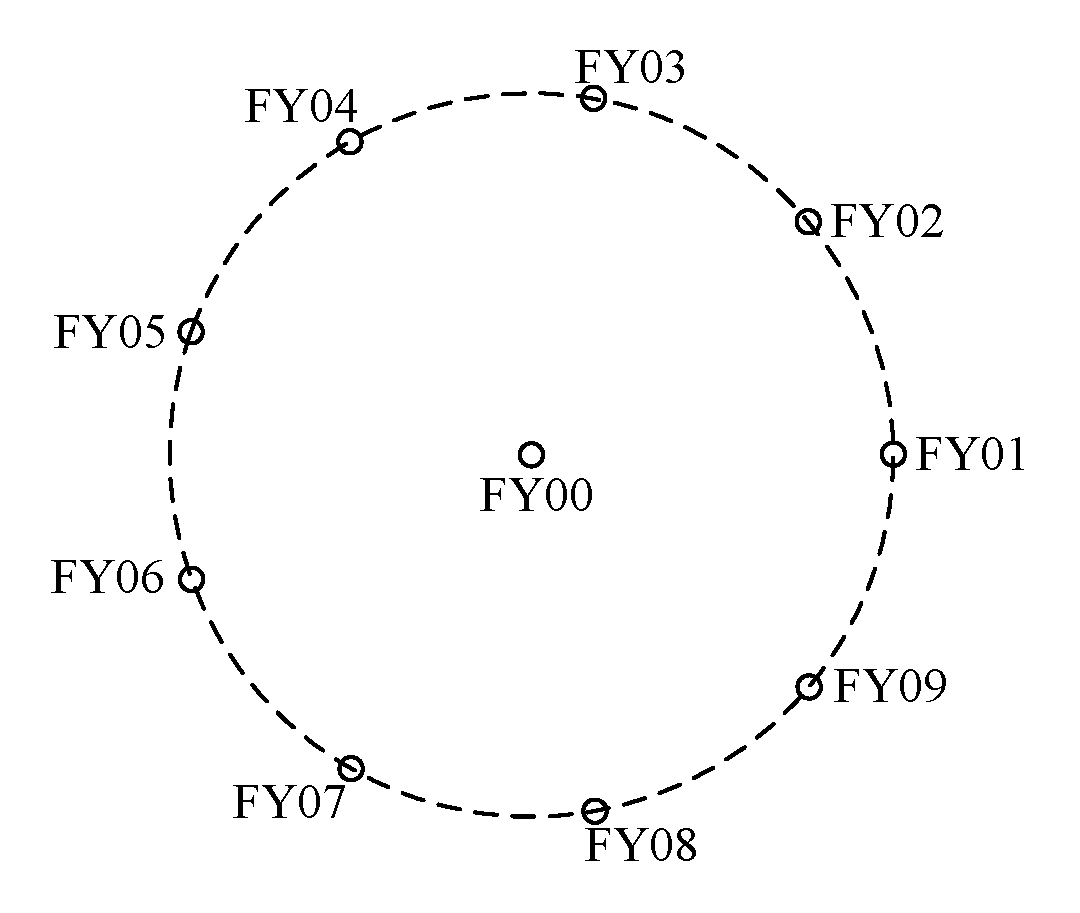
\includegraphics[width=\textwidth]{图片/无人机以及编号示意图.pdf}
        \caption{圆周无人机编队以及编号示意图}
        \label{fig:编号示意图}
    \end{minipage}
    \begin{minipage}[t]{0.48\textwidth}
        \centering
        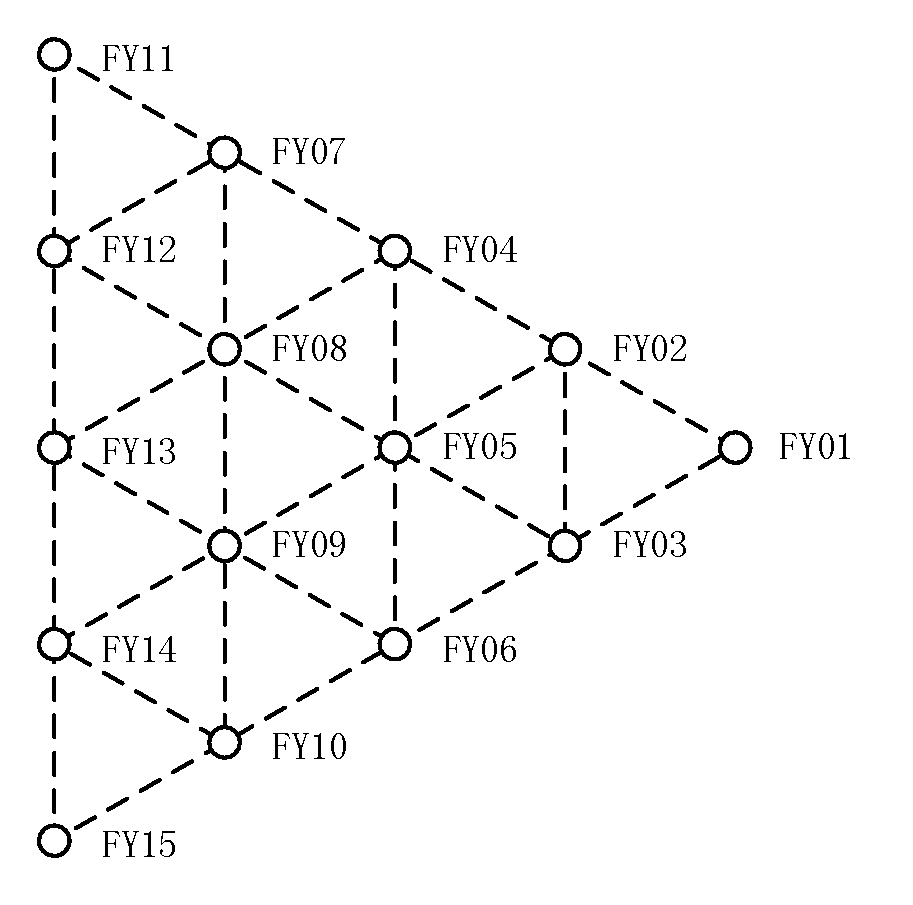
\includegraphics[width=\textwidth]{图片/锥形队列.pdf}
        \caption{锥形无人机编队以及编号示意图}
        \label{fig:锥形编队}
    \end{minipage}
\end{figure}

对此,题目要求我们完成以下任务:
\begin{enumerate*}
    \item 位于圆心的一架飞机和位于圆周的两架飞机发射信号。接受信号的无人机可以接收到该无人机和圆周上发射信号无人机的连线,与该无人机和位于圆心的无人机连线之间的夹角。假设发射信号的无人机位置精确,接受信号的无人机位置略有偏差。建立接受信号无人机的定位模型,确定无人机的位置。
    \item 某位置略有偏差的无人机接收到FY00和FY01的信号,假设发射信号的无人机位置无偏差,其需要再接受几架编号位置的其他无人机发射的信号,才能实现无人机位置的准确定位。
    \item 按编队要求,1架无人机位于圆心,另9架无人机均匀分布在半径为100 m的圆周上,但初始位置略有偏差。需要我们给出调整方案,通过多次的迭代调整,使得最终外围的9架无人机可以均匀分布在某个圆周上。每次调整我们可以选择圆心和圆周上的三架无人机发射信号,其余无人机接收信号,根据接收到的方向信息进行自我位置调整。
\end{enumerate*}

之后,我们关注一个如图\ref{fig:锥形编队}所示的锥形编队。题目要求我们,仍然考虑无源定位的情况,并给出调整的方案。

%%%%%%%%%%%%%%%%%%%%%%%%%%%%%%%%%%%%%%%%%%%%%%%%%%%%%%%%%%%%%%%%
%                                                              %
%%%%%%%%%%%%%%%%%%%%%%%%%%%%%%%%%%%%%%%%%%%%%%%%%%%%%%%%%%%%%%%%

\section{基本假设}

我们有如下的基本假设:
\begin{itemize*}
    \item 无人机之间的信息不能共享;
    \item 发射信号的无人机不能同时接收信号;
    \item 每一架无人机都知道自己的编号;
    \item 每一架无人机都知道不同编号无人机的相对位置关系;
    \item 除特殊要求外(问题一第2小问),接收信号的无人机知道每一个接收的角度信息来源于哪两架无人机;
    \item 在以FY00为原点的极坐标系中,圆周上无人机的极角偏差小于$\frac{1}{18}\pi$;
    \item 无人机只能接收角度信息,也只能依靠角度的信息来引导自己的移动,其基本移动模式为,接收两个角度信号,保持一个角度不变,调整自身位置使得另一个角度为目标数值;
\end{itemize*}

%%%%%%%%%%%%%%%%%%%%%%%%%%%%%%%%%%%%%%%%%%%%%%%%%%%%%%%%%%%%%%%%
%                                                              %
%%%%%%%%%%%%%%%%%%%%%%%%%%%%%%%%%%%%%%%%%%%%%%%%%%%%%%%%%%%%%%%%

\section{符号说明}

见表\ref{tab:符号说明}。表中列举了全文中的常用符号,部分符号在全文中会有不同的含义,这些符号在会在使用时进行说明。

\begin{table}[!ht]
    \centering
    \caption{本文所用符号说明}
    \label{tab:符号说明}
    \begin{tabular}{ccc}
        \toprule
        符号  &  符号说明 & 备注\\
        \midrule
        $r_0$ & 无人机编队的圆半径 & ——\\
        FY0N  & 序号为$n$的无人机 & 可用其他字母替代\\
        $\alpha_{ABC}$ & FY0B接收的来自于FY0A和FY0C的角信号 & 可用数字或其他字母替代\\
        $\theta_{ABC}$ & FY0A、FY0B、FY0C三点共圆的圆心极角& 可用数字或其他字母替代\\
        $\rho_{ABC}$ & FY0A、FY0B、FY0C三点共圆的圆心极径& 可用数字或其他字母替代\\
        $d_{i}$ & FY0I当前位置与正确位置间的距离 & 可用数字或其他字母替代\\
        \bottomrule
    \end{tabular}
\end{table}

%%%%%%%%%%%%%%%%%%%%%%%%%%%%%%%%%%%%%%%%%%%%%%%%%%%%%%%%%%%%%%%%
%                                                              %
%%%%%%%%%%%%%%%%%%%%%%%%%%%%%%%%%%%%%%%%%%%%%%%%%%%%%%%%%%%%%%%%

\section{问题一(1):接受信号无人机的定位模型}

\subsection{基于两圆相交的定位模型}

由于圆的对称性,我们不妨设其中一个发射信号的无人机为FY01。如图\ref{fig:问题1-1示意图}所示,位于圆心的FY00、位于圆周的FY01和另一架位于圆周但序数任意的无人机FY0M发射信号,FY0N接受信号。

\begin{figure}[!ht]
    \centering
    \begin{minipage}[t]{0.48\textwidth}
        \centering
        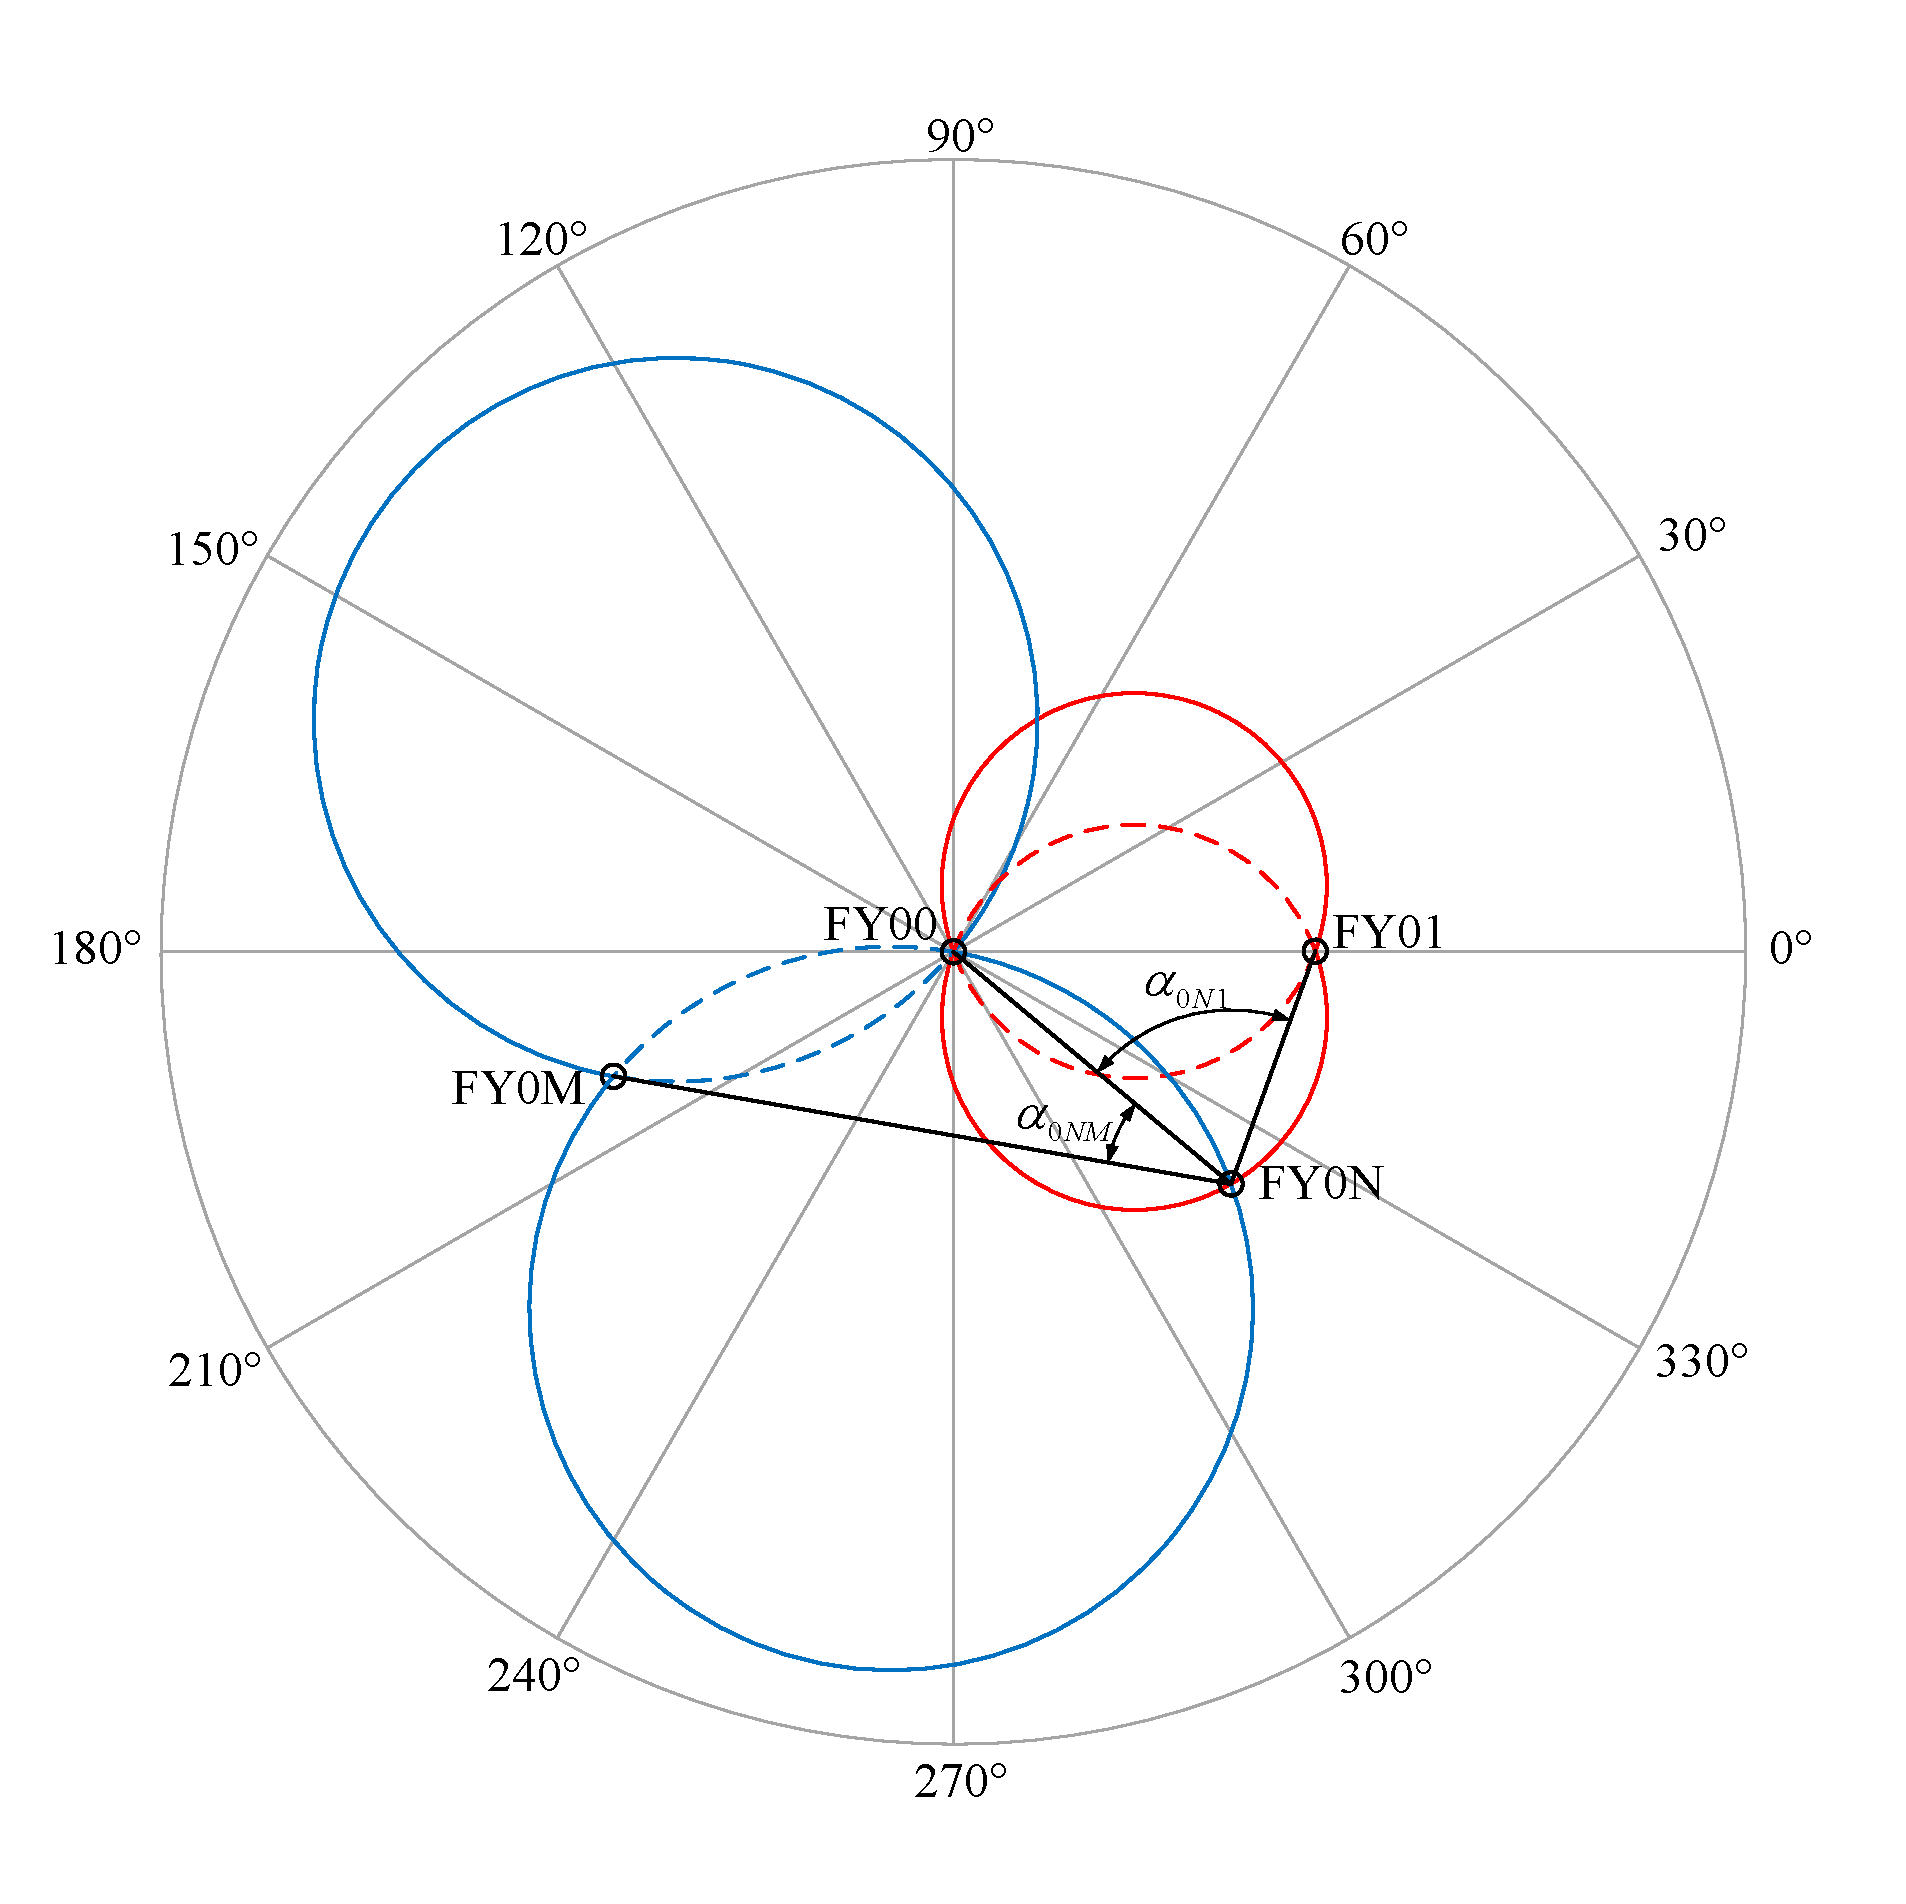
\includegraphics[width=\textwidth]{图片/问题1-1示意图.pdf}
        \caption{接受信号无人机的定位模型}
        \label{fig:问题1-1示意图}
    \end{minipage}
    \begin{minipage}[t]{0.48\textwidth}
        \centering
        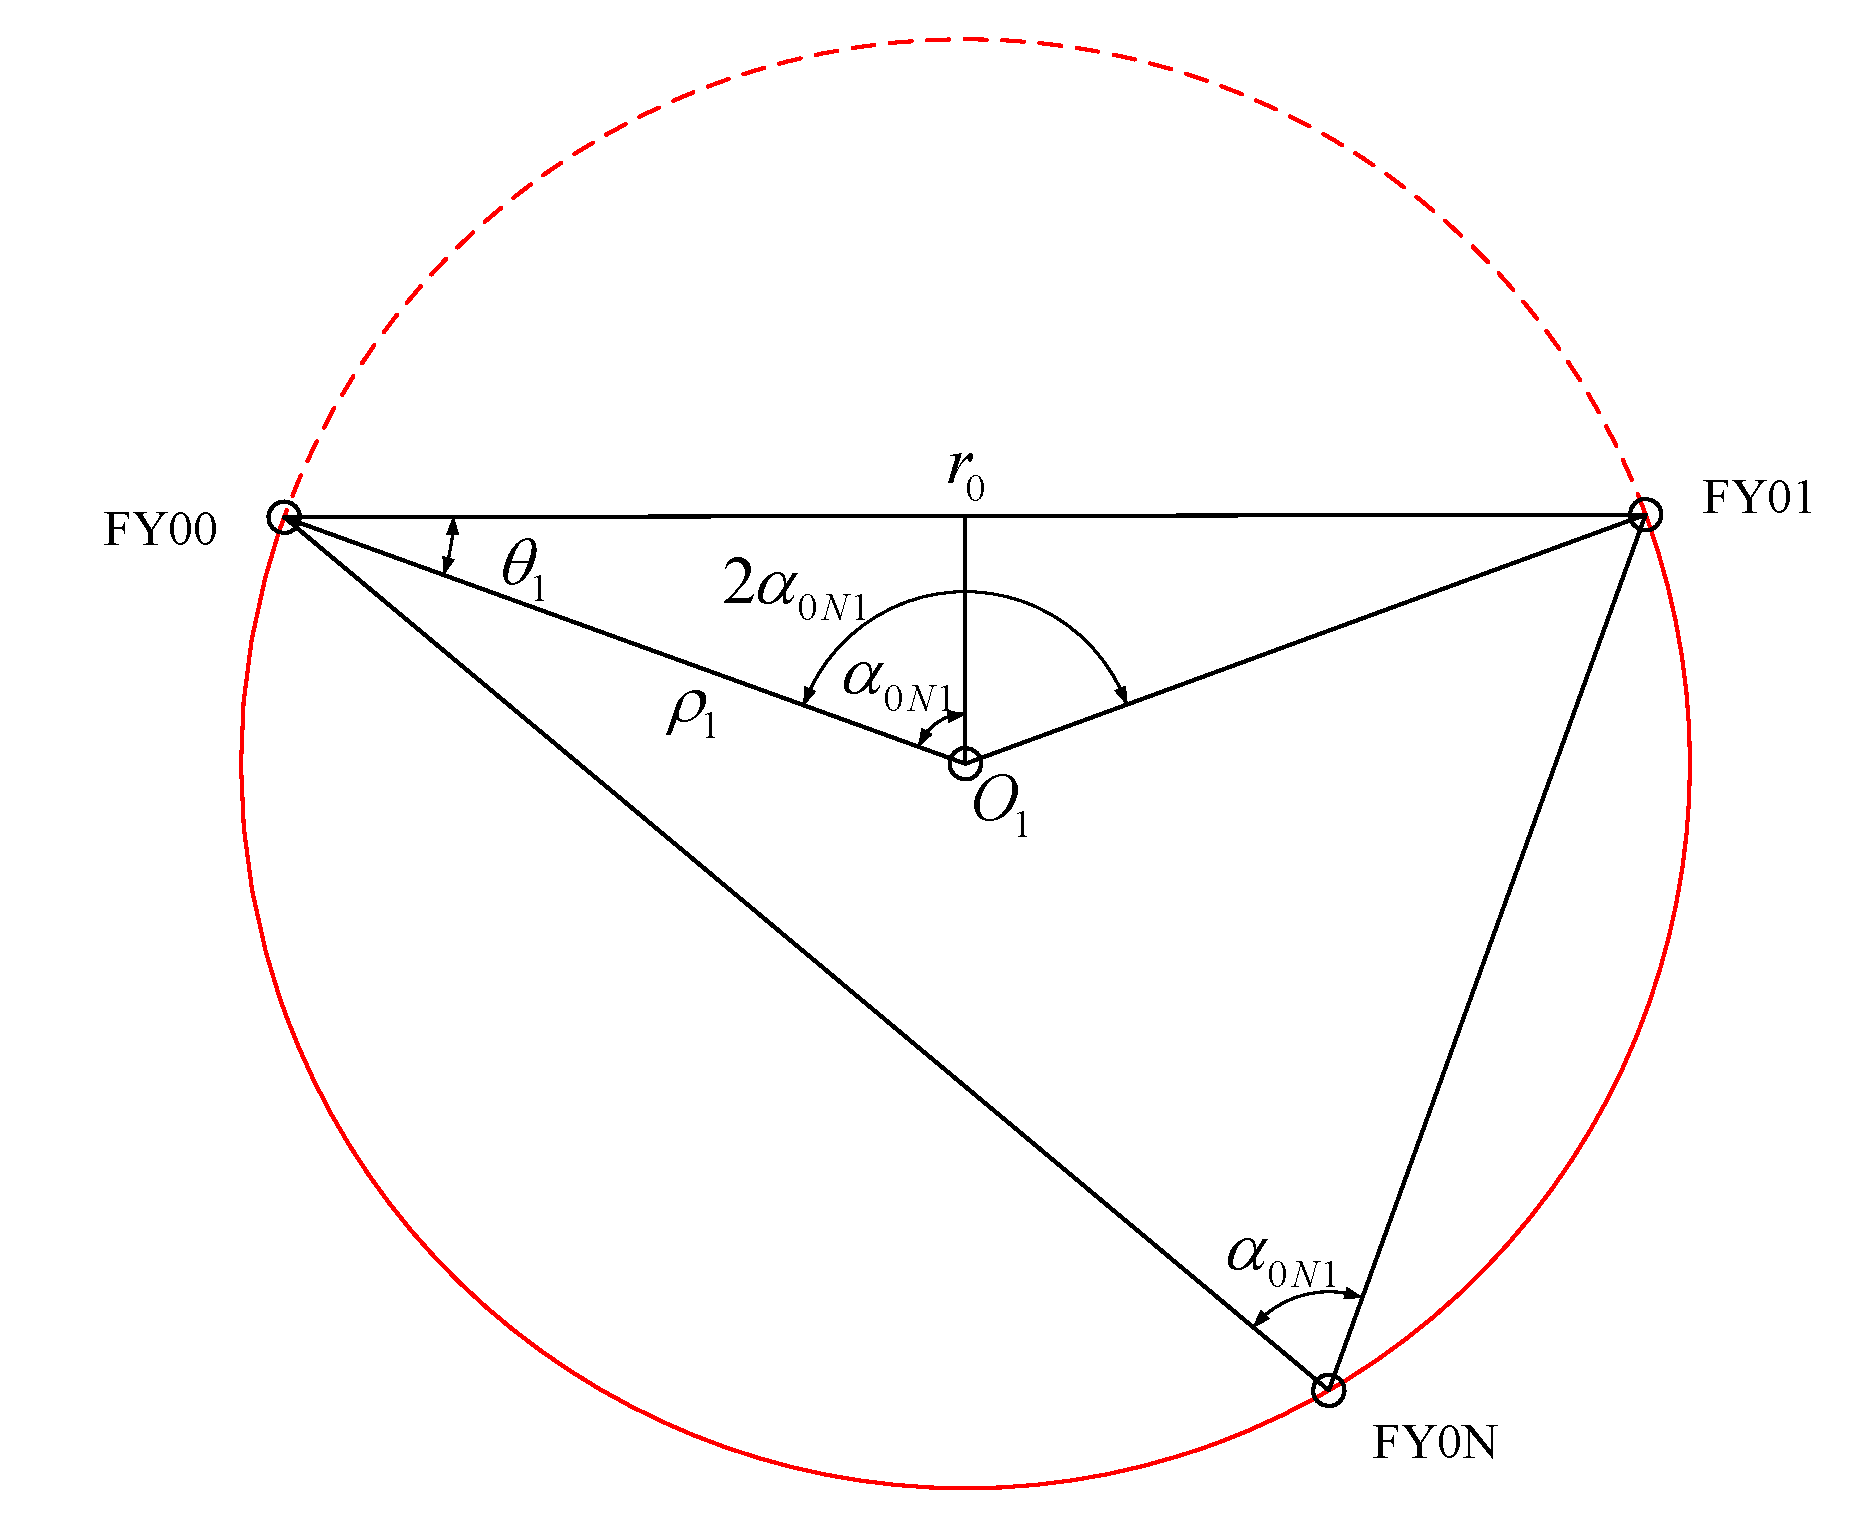
\includegraphics[width=\textwidth]{图片/问题1-1示意图 - 局部.pdf}
        \caption{单个圆的几何分析}
        \label{fig:单个圆的几何分析}
    \end{minipage}
\end{figure}

FY0N可以接收到两个角度信号$\alpha_{0N1}$和$\alpha_{0NM}$。根据简单的几何知识(圆周角相等)我们可以知道,满足$\alpha_{0N1}$为固定值的所有点都在图\ref{fig:问题1-1示意图}中所示的红色实线上,其是两段圆弧组合而成。同理,满足$\alpha_{0NM}$为固定值的所有点都在图\ref{fig:问题1-1示意图}中所示的蓝色实线上。

我们取FY00为极点,FY00为起点指向FY01的射线为极轴,构建极坐标系,设FY0M的序数为$m$。设FY01的极坐标为$\left(r_0,0\right)$,则FY0M的极坐标为$\left(r_0,\frac{2}{9}\left(m-1\right)\pi\right)$。其中,$r_0$为无人机编队所在圆的半径。

接下来,我们以红色下半部分圆弧为例,来讨论圆心的坐标,其局部图如图\ref{fig:单个圆的几何分析}所示。从中我们可以得到,确定圆心坐标的两个重要的参数:
\begin{align}
    \rho_1 &= \frac{r_0}{2\sin \alpha_{0N1}}\\
    \theta_1 &= \frac{\pi}{2} - \alpha_{0N1}
\end{align}
这样,我们可以得到$O_1$的极坐标为:
\begin{equation}
    A = \left(\rho_1,-\theta_1\right) = \left(\frac{r_0}{2\sin \alpha_{0N1}}, - \frac{\pi}{2} + \alpha_{0N1}\right)
\end{equation}

同理,我们可以得到与其对应的圆的圆心坐标,以及蓝色圆弧的圆心坐标。设FY00,FY01和FY0N组成的圆的圆心坐标为$A_{0N1}$,FY00,FY0M和FY0N组成的圆的圆心坐标为$A_{0NM}$,则其可以表示为:
\begin{align}
    A_{0N1} &= \left(\frac{r_0}{2\sin \alpha_{0N1}}, 0 \pm \left(\frac{\pi}{2} - \alpha_{0N1}\right)\right)\\
    A_{0NM} &= \left(\frac{r_0}{2\sin \alpha_{0NM}}, \frac{2}{9}\left(m-1\right)\pi \pm \left(\frac{\pi}{2} - \alpha_{0NM}\right)\right)\label{eq:0NM圆心坐标}
\end{align}

接下来,我们求取圆在极坐标系下的方程。我们知道,极坐标下,圆心在$(\rho_0,\theta_0)$,半径为$r_0$的圆的一般方程为:
\begin{equation}
    \rho^2 + \rho_0^2 - 2\rho\,\rho_0\cos\left(\theta - \theta_0\right) = r_0^2
\end{equation}

我们将两个圆的信息带入,可以得到如下方程组:
\begin{equation}
    \left\{
    \begin{aligned}
        \rho^2 + \rho_{0N1}^2 - 2\rho\,\rho_{0N1}\cos\left(\theta - \theta_{0N1}\right) &= \rho_{0N1}^2\\
        \rho^2 + \rho_{0NM}^2 - 2\rho\,\rho_{0NM}\cos\left(\theta - \theta_{0NM}\right) &= \rho_{0NM}^2
    \end{aligned}
    \right.
\end{equation}

整理可以得到(显然原点是一个解,我们不考虑原点的情况,所以将$\rho$约去):

\begin{equation}
    \label{eq:方程组}
    \left\{
    \begin{aligned}
        \rho &= \frac{r_0}{\sin \alpha_{0N1}}\left(\cos\theta\,\cos\theta_{0N1} + \sin\theta\,\sin\theta_{0N1}\right)\\
        \rho &= \frac{r_0}{\sin \alpha_{0NM}}\left(\cos\theta\,\cos\theta_{0NM} + \sin\theta\,\sin\theta_{0NM}\right)
    \end{aligned}
    \right.
\end{equation}

整理可以得到:
\begin{equation}
    \cos\theta\frac{\cos\theta_{0N1}}{\sin\alpha_{0N1}} - \cos\theta\frac{\cos\theta_{0NM}}{\sin\alpha_{0NM}} =
    \sin\theta\frac{\sin\theta_{0NM}}{\sin\alpha_{0NM}} - \sin\theta\frac{\sin\theta_{0N1}}{\sin\alpha_{0N1}}
\end{equation}

进一步化简可以得到:
\begin{equation}
    \tan\theta = \frac
    {\frac{\cos\theta_{0N1}}{\sin\alpha_{0N1}} - \frac{\cos\theta_{0NM}}{\sin\alpha_{0NM}}}
    {\frac{\sin\theta_{0NM}}{\sin\alpha_{0NM}} - \frac{\sin\theta_{0N1}}{\sin\alpha_{0N1}}}
    \label{eq:tantheta表达式}
\end{equation}
从图\ref{fig:编号示意图}中可以看出,在无人机的位置仅略有偏差的情况下,应该不会出现在$\tan\theta$的值不存在的情况(这要求FY03和FY08的偏移不能超过10度),我们这里使用$\tan\theta$的值来确定无人机的位置是合理的。

得到FY0N的在极坐标系下的角度信息后,我们将其带回式\ref{eq:方程组}中任意一个式子,就可以得到$\rho$的取值。比如:
\begin{equation}
    \rho = \frac{r_0}{\sin \alpha_{0N1}}\left(\cos\theta\,\cos\theta_{0N1} + \sin\theta\,\sin\theta_{0N1}\right)
    \label{eq:极径计算}
\end{equation}

接下来,我们所需要解决的还有两个问题:
\begin{enumerate*}
    \item $\theta_{0N1}$和$\theta_{0NM}$的取值有两个,我们需要确定选择哪一个;
    \item 在$0$到$2\pi$范围内,有两个$\theta$的取值使得$\tan\theta$为某一特定值,我们需要确定选择哪一个。
\end{enumerate*}

\subsection{特定情况下的讨论}

首先,我们来确定$\theta_{0N1}$和$\theta_{0NM}$的具体取值。那么我们首先要讨论$\alpha_{0N1}$和$\alpha_{0NM}$的取值范围。

\begin{figure}[!ht]
    \centering
    \begin{minipage}[t]{0.48\textwidth}
        \centering
        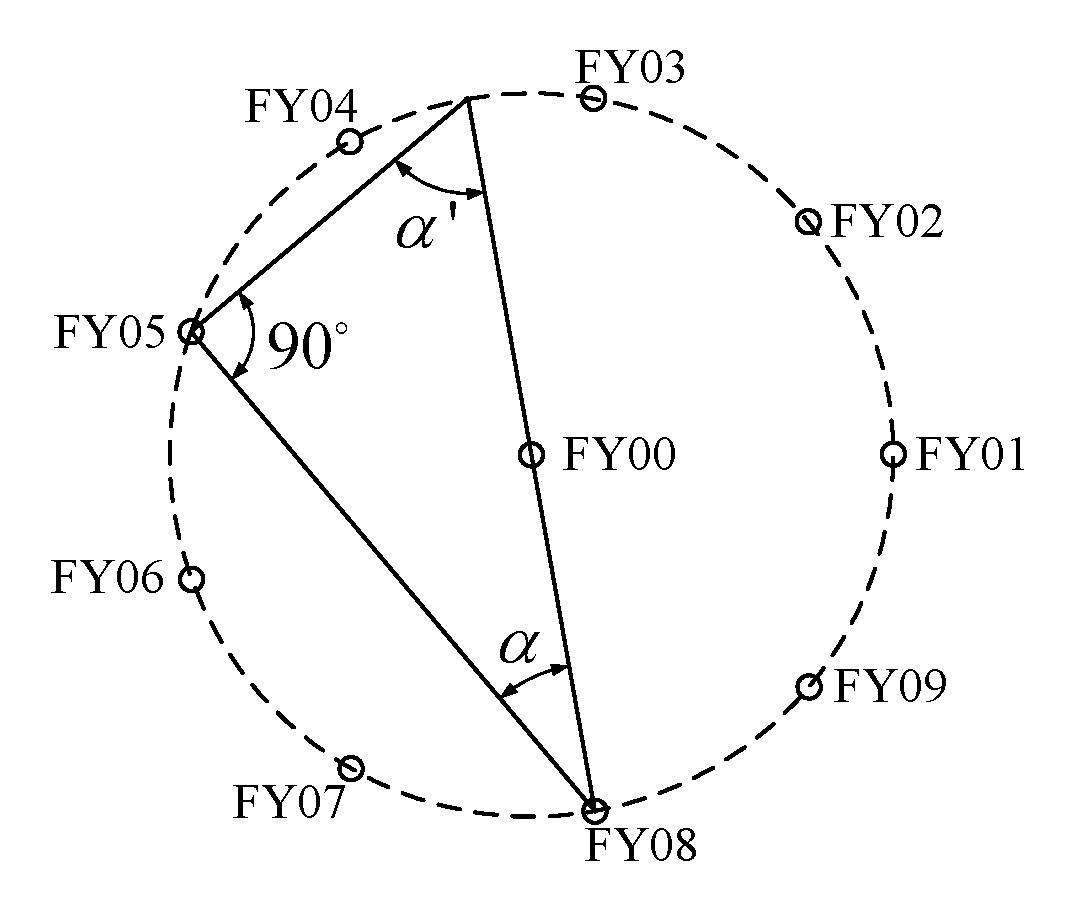
\includegraphics[width=\textwidth]{图片/角度范围示意图.pdf}
        \caption{$\alpha$取值范围示意图}
        \label{fig:角度范围示意图}
    \end{minipage}
    \begin{minipage}[t]{0.48\textwidth}
        \centering
        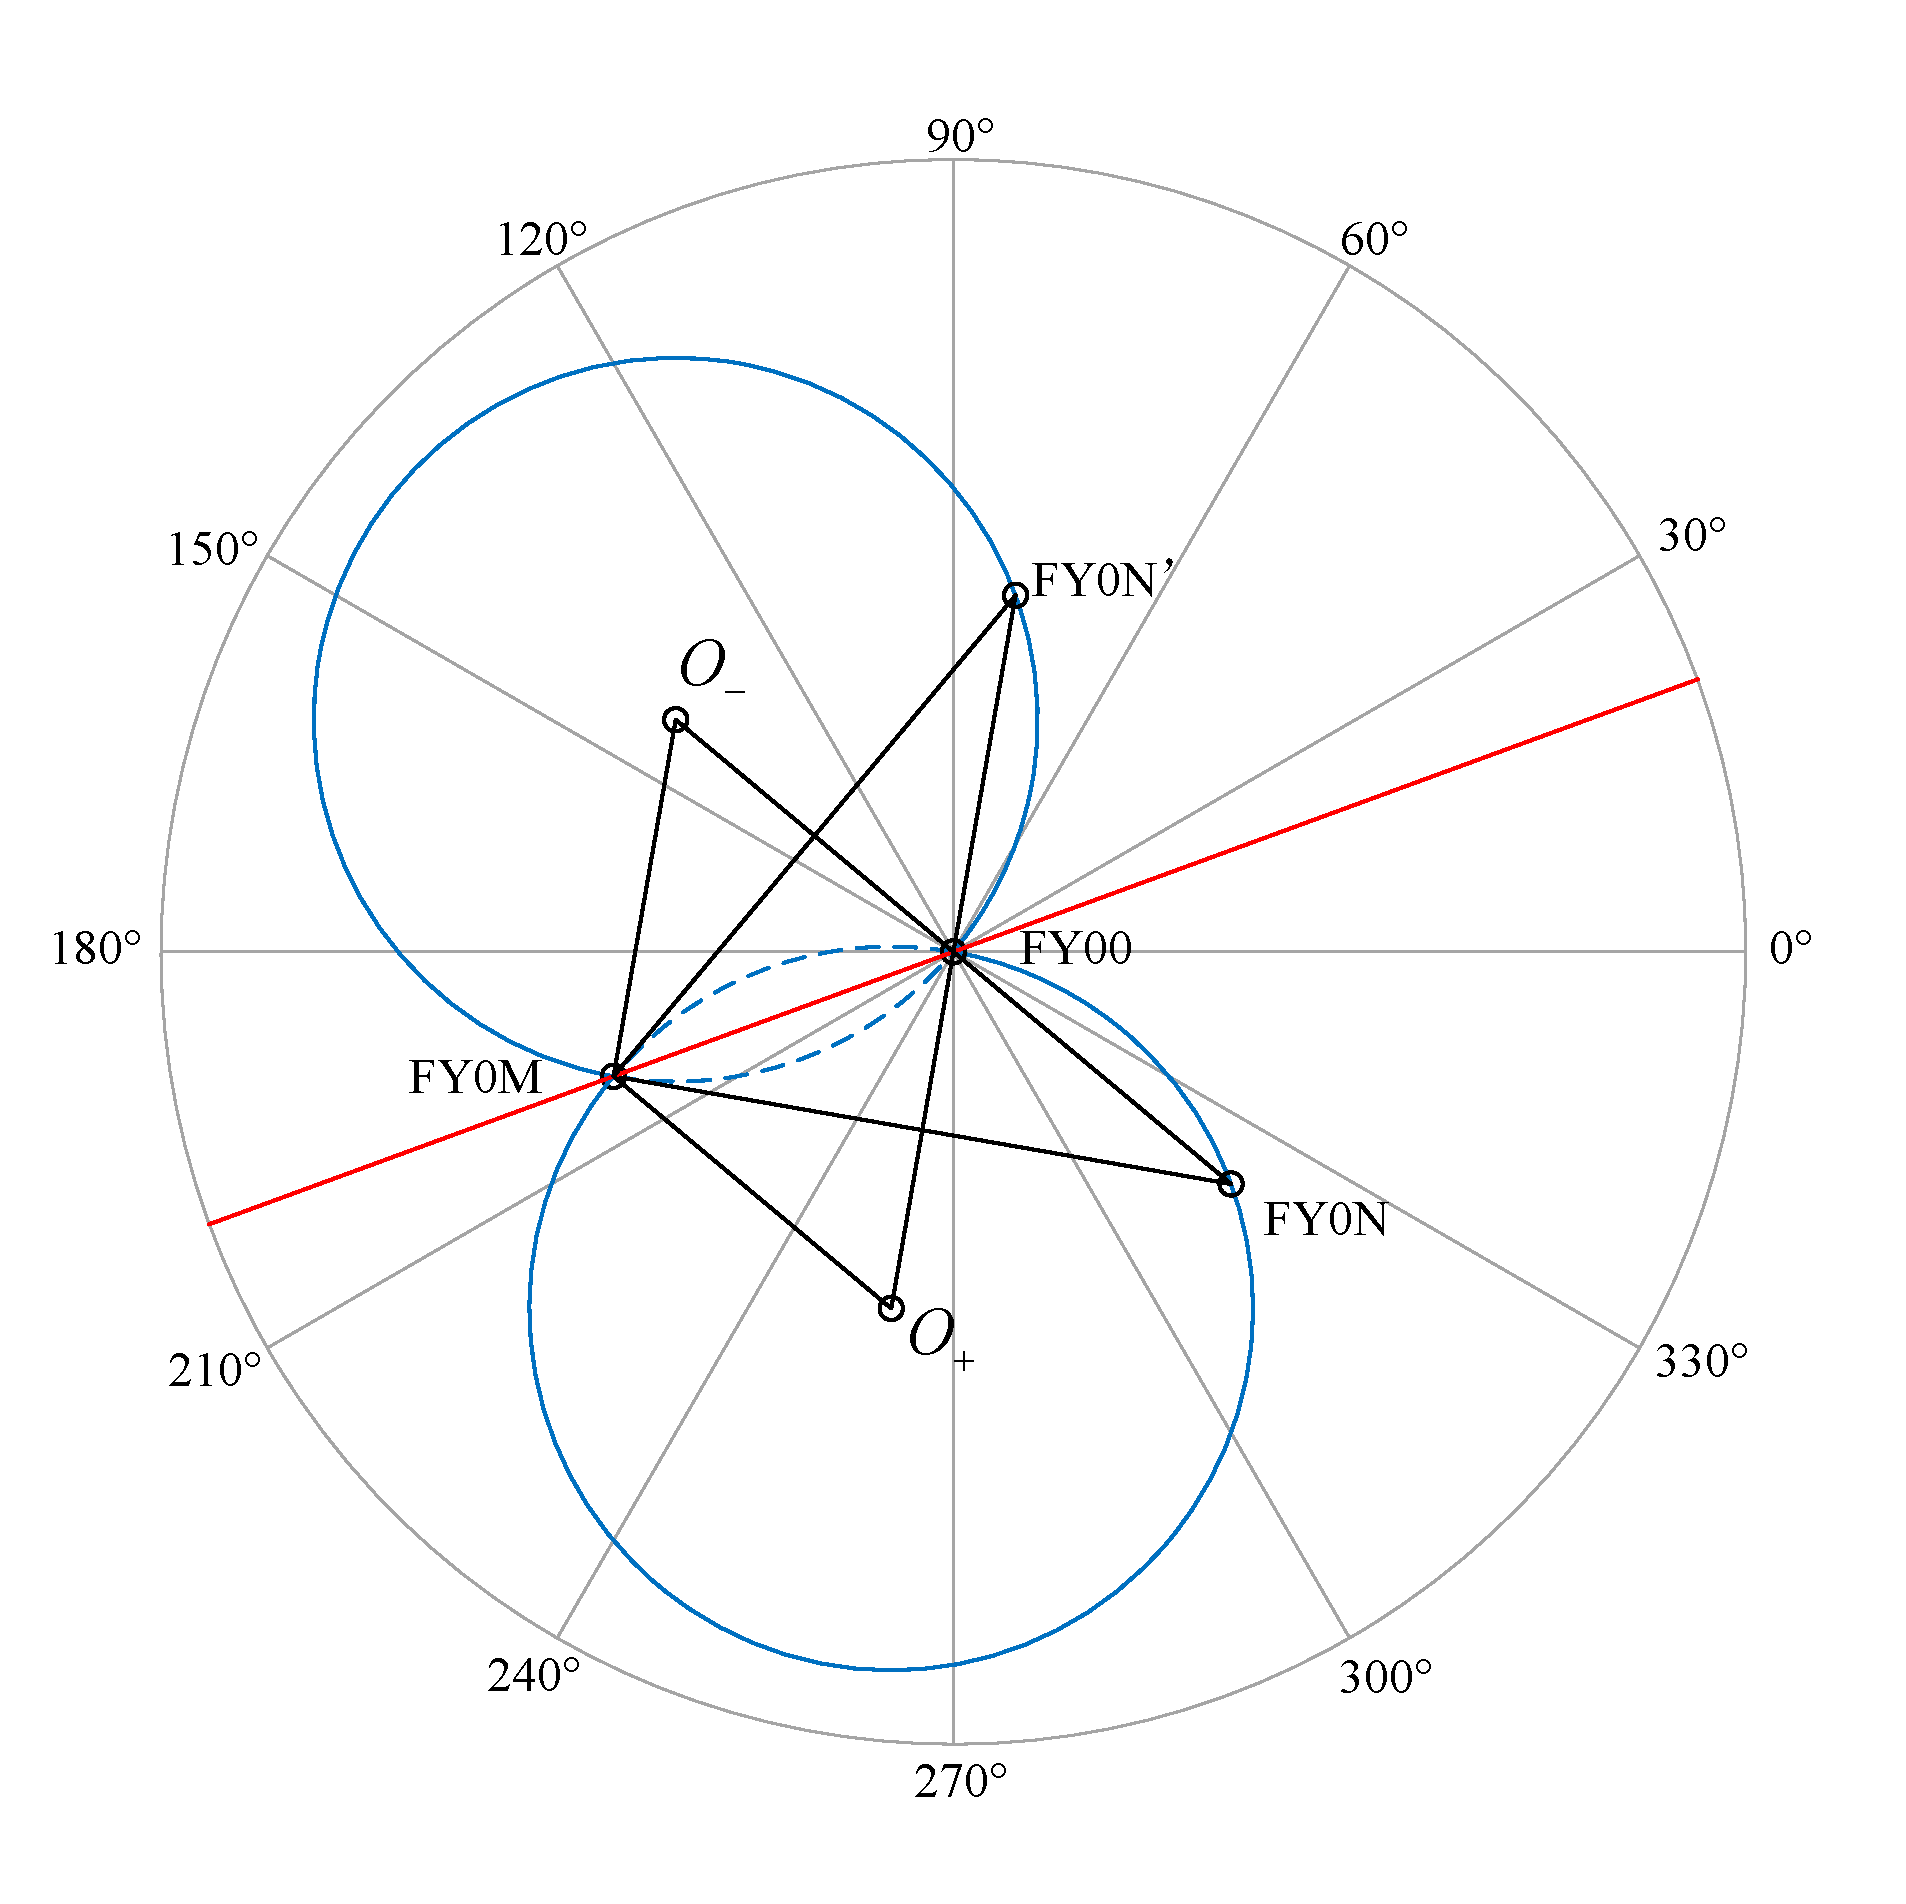
\includegraphics[width=\textwidth]{图片/theta取值讨论.pdf}
        \caption{$\theta$取值示意图}
        \label{fig:正负取值示意图}
    \end{minipage}
\end{figure}

如图\ref{fig:角度范围示意图}所示,对于任意的一个$\alpha$,我们都会有:
\begin{equation}
    \alpha+\alpha ' = \frac{\pi}{2}
\end{equation}
又显然有$\alpha$和$\alpha '$都是大于0的,所以
\begin{equation}
    0 < \alpha < \frac{\pi}{2}
\end{equation}
这对于,所有的圆周上无人机所接收到的角度信号都是成立的,所以:
\begin{align}
    0 &< \alpha_{0N1} < \frac{\pi}{2}\\
    0 &< \alpha_{0NM} < \frac{\pi}{2}
\end{align}

现在我们观察图\ref{fig:正负取值示意图}。我们从中可以看到,对于$\theta_{0NM}$来说,$\frac{2}{9}\left(m-1\right)\pi \pm \left(\frac{\pi}{2} - \alpha_{0NM}\right)$中取$+$还是$-$,取决于,FY0N位于FY0M和FY00连成的直线(图\ref{fig:正负取值示意图}中红色直线)的上方或者是下方(当正好位于直线上时,外接圆不存在)。设FY0N在极坐标系下的极角为$\theta_n$用数学语言表达就是:

\begin{equation}
    \theta_{0NM} = \left\{
    \begin{aligned}
        & \frac{2}{9}\left(m-1\right)\pi + \left(\frac{\pi}{2} - \alpha_{0NM}\right)&&,
        0 < \theta_n - \frac{2}{9}\left(m-1\right)\pi + 2k\pi< \pi\\
        & \frac{2}{9}(m-1)\pi - \left(\frac{\pi}{2} - \alpha_{0NM}\right)&&,
        \pi < \theta_n - \frac{2}{9}(m-1)\pi + 2k\pi < 2\pi
    \end{aligned}
    \right.
    \label{eq:theta分类讨论}
\end{equation}
其中,$k \in \mathbb{Z}$。

如果我们认为略有偏差的位置,不会影响FY0N与直线的位置关系(这里要求相当宽松,仅要求偏差小于20°)。我们设FY0N无人机所对应的序数为$n$,则$\theta_n=\frac{2}{9}(n-1)\pi$,将其带入式\ref{eq:theta分类讨论}。可以得到:

\begin{equation}
    \theta_{0NM} = \left\{
    \begin{aligned}
        & \frac{2}{9}\left(m-1\right)\pi + \left(\frac{\pi}{2} - \alpha_{0NM}\right)&&,
        0 < n - m + 9k < \frac{9}{2}\\
        & \frac{2}{9}\left(m-1\right)\pi - \left(\frac{\pi}{2} - \alpha_{0NM}\right)&&,
        \frac{9}{2} < n - m + 9k < 9
    \end{aligned}
    \right.
    \label{eq:theta分类讨论最终结果}
\end{equation}

同理,我们可以得到$\theta_{0N1}$在不同情况下的取值,将$m$为1带入式\ref{eq:theta分类讨论最终结果}中即可。表\ref{tab:theta取值}展示了对于不同的$n$和$m$,$\theta_{0N1}$和$\theta_{0NM}$的取值。

\begin{table}[!ht]
    \centering
    \caption{$\theta_{0N1}$和$\theta_{0NM}$的取值}
    \label{tab:theta取值}
    \small
    \begin{tabular}{ccc}
        \toprule
        ~  &  $1 \leq n - m + 9k \leq 4$ & $5 \leq n - m + 9k \leq 8$\\
        \midrule
        $2 \leq n \leq 5$ & 
        $
        \left\{
        \begin{aligned}
            \theta_{0N1} &= \frac{\pi}{2} - \alpha_{0N1}\\
            \theta_{0NM} &= \frac{2}{9}\left(m-1\right)\pi + \left(\frac{\pi}{2} - \alpha_{0NM}\right)
        \end{aligned}
        \right.
        $
        & 
        $
        \left\{
        \begin{aligned}
            \theta_{0N1} &= \frac{\pi}{2} - \alpha_{0N1}\\
            \theta_{0NM} &= \frac{2}{9}\left(m-1\right)\pi - \left(\frac{\pi}{2} - \alpha_{0NM}\right)
        \end{aligned}
        \right.
        $
        \\
        $6 \leq n \leq 9$ &
        $
        \left\{
        \begin{aligned}
            \theta_{0N1} &= - \frac{\pi}{2} + \alpha_{0N1}\\
            \theta_{0NM} &= \frac{2}{9}\left(m-1\right)\pi + \left(\frac{\pi}{2} - \alpha_{0NM}\right)
        \end{aligned}
        \right.
        $
        & 
        $
        \left\{
        \begin{aligned}
            \theta_{0N1} &= - \frac{\pi}{2} + \alpha_{0N1}\\
            \theta_{0NM} &= \frac{2}{9}\left(m-1\right)\pi - \left(\frac{\pi}{2} - \alpha_{0NM}\right)
        \end{aligned}
        \right.
        $
        \\
        \bottomrule
    \end{tabular}
\end{table}

接下来,我们还需要通过$\tan\theta$的值来确定$\theta$的取值。不能直接使用$\arctan\tan\theta$来确定$\theta$的值,因为$\arctan$函数的值域是$\left(-\frac{\pi}{2},\frac{\pi}{2}\right)$,而我们需要的$\theta$的值域是$\left(0,2\pi\right)$。在无人机的位置仅仅略有偏差(这里要求偏差小于10°,否则会出现跨区域问题)的情况下,我们可以通过$n$的取值,来判断$\theta$的取值范围,然后再通过$\tan\theta$的值来确定$\theta$的具体取值。如表\ref{tab:thetan取值}所示。

\begin{table}[!ht]
    \centering
    \caption{$\theta$的取值}
    \label{tab:thetan取值}
    \begin{tabular}{cc}
        \toprule
        ~  &  $\theta$\\
        \midrule
        $n=2,3$ & $\arctan\tan\theta$\\
        $n=4,5,6,7$ & $\arctan\tan\theta + \pi$\\
        $n=8,9$ & $\arctan\tan\theta + 2\pi$\\
        \bottomrule
    \end{tabular}
\end{table}

综上所述,在无人机位置的偏差角度小于10°的情况下,我们完成了题目要求的无人机的定位模型。

%%%%%%%%%%%%%%%%%%%%%%%%%%%%%%%%%%%%%%%%%%%%%%%%%%%%%%%%%%%%%%%%
%                                                              %
%%%%%%%%%%%%%%%%%%%%%%%%%%%%%%%%%%%%%%%%%%%%%%%%%%%%%%%%%%%%%%%%

\section{问题一(2):无人机有效定位条件}

\subsection{通过角度信息估算发射信号无人机序数}

对于任意两个无人机,假设其编号分别为$n$和$m$,则如图\ref{fig:问题1-2示意图1}所示。

\begin{figure}[!ht]
    \centering
    \begin{minipage}[t]{0.48\textwidth}
        \centering
        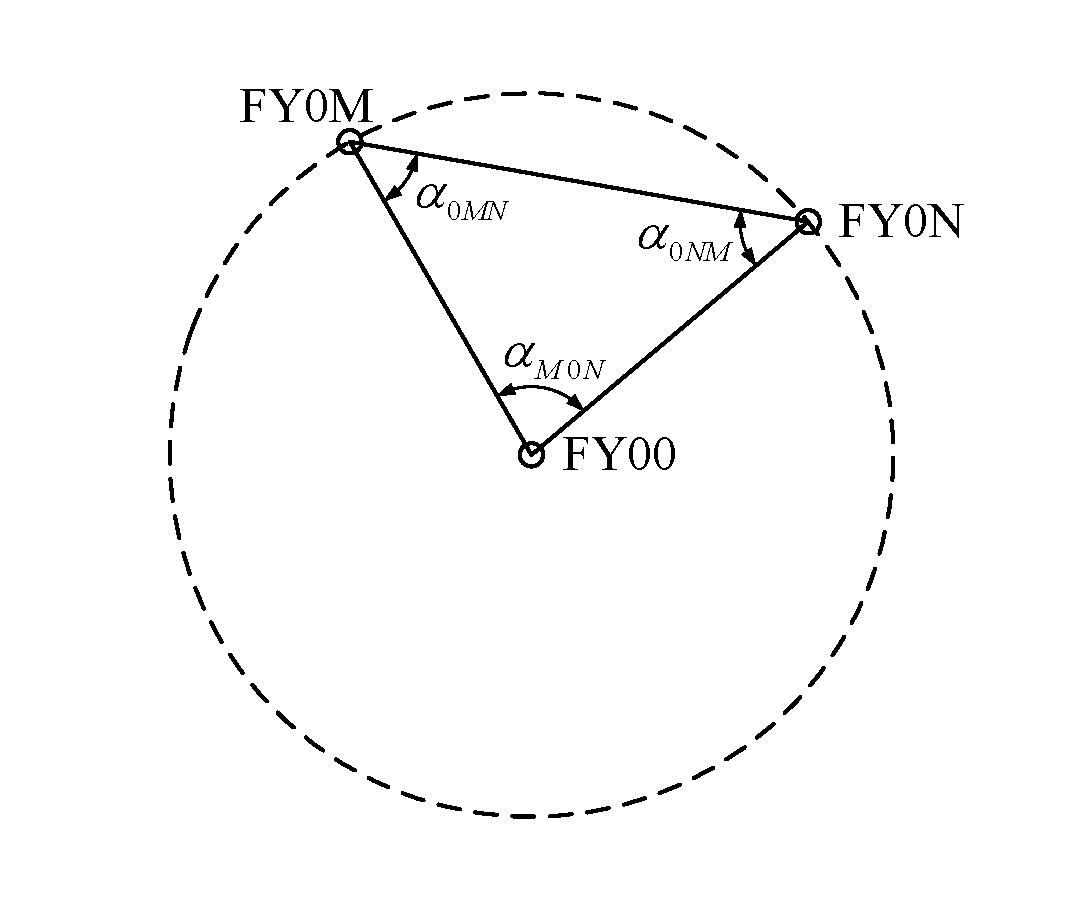
\includegraphics[width=\textwidth]{图片/问题1-2示意图1.pdf}
        \caption{两圆周无人机角度关系}
        \label{fig:问题1-2示意图1}
    \end{minipage}
    \begin{minipage}[t]{0.48\textwidth}
        \centering
        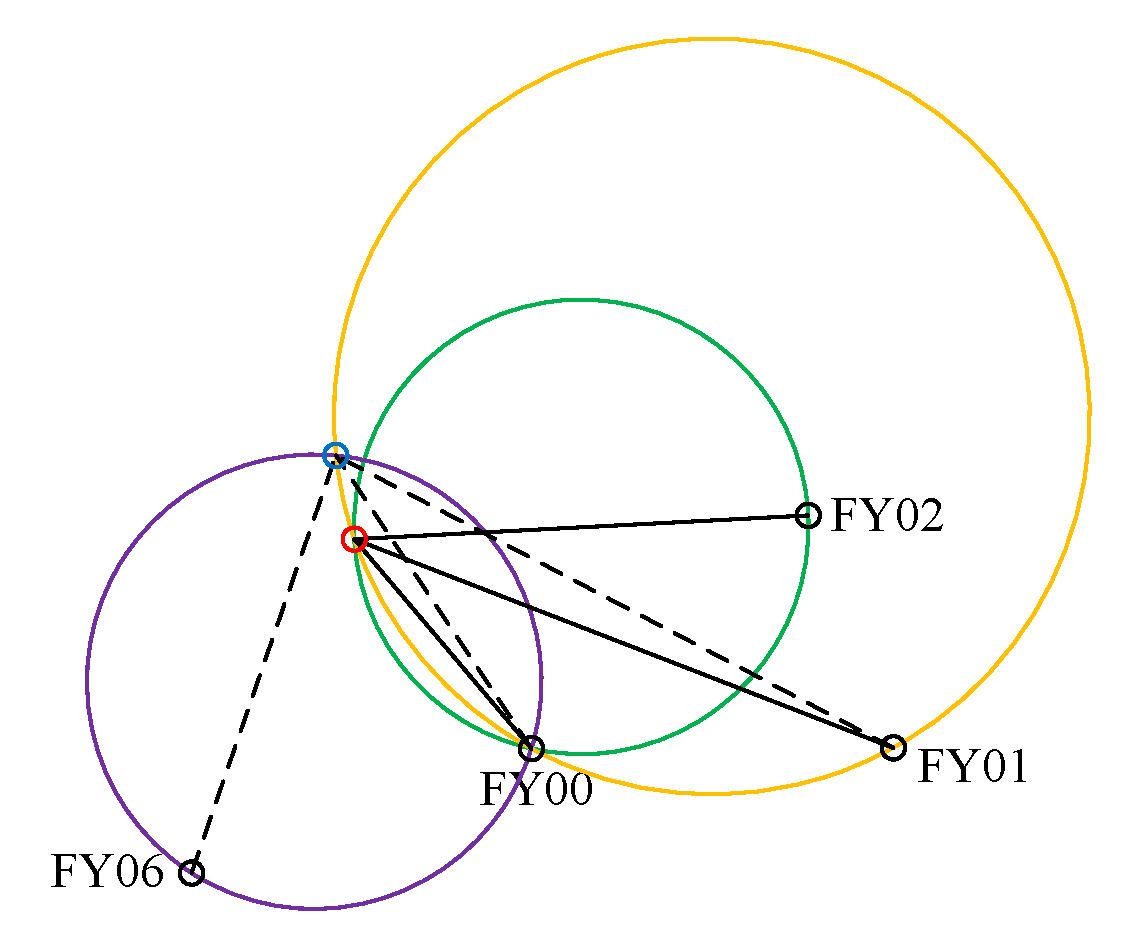
\includegraphics[width=\textwidth]{图片/问题1-2示意图2.pdf}
        \caption{仅有额外1架飞机的情况}
        \label{fig:额外1架飞机}
    \end{minipage}
\end{figure}

如果,FY0M和FY0N的位置是准确的,因为9架无人机均匀分布在圆周上,我们可以得到:
\begin{equation}
    \alpha_{M0N} = \frac{2}{9}\pi\left|n-m\right|
\end{equation}

根据等腰三角形的性质,我们很容易可以得到:
\begin{equation}
    \alpha_{0MN} = \alpha_{0NM} = \frac{1}{2}\pi - \frac{1}{9}\pi\left|n-m\right|
\end{equation}

通过上面的式子,即使在FY0M和FY0N的位置略有偏差的情况下,我们也可以通过$\alpha_{0MN}$和$\alpha_{0NM}$的值,来估计$|n-m|$的值。我们以$\alpha_{0MN}$为例,我们可以得到:
\begin{equation}
    \left|n-m\right| \approx 9\left(\frac{1}{2} - \frac{\alpha_{0MN}}{\pi}\right)
    \label{eq:估计nm}
\end{equation}

为了使得对$\left|n-m\right|$的估计不出现错误,$\alpha_{0MN}$的误差应当小于$\frac{1}{18}\pi$,也就是:
\begin{equation}
    \Delta\alpha_{0MN} < \frac{1}{18}\pi
    \label{eq:误差条件}
\end{equation}
接下来的讨论都将以此为基础。

显然,对于一个$m$,有两个$n$的可能取值满足条件,分别记为$n_1$和$n_2$,为了简化后续叙述,我们称FY0N1与FY0N2关于FY0M对称。

\subsection{额外一架无人机的情况}

现在我们来讨论,如图\ref{fig:额外1架飞机}所示的情况。FY04的位置略有偏差,其实际位置位于图中红色圆圈标识的位置。其接收到了FY00和FY01所提供的角度信息,结合自身的序号,知道了自身位于橙色的圆周上。同时其接收到了一个未知来源的(实际来源于FY02),角度约为$\frac{7}{18}\pi$的角度信息。其通过式\ref{eq:估计nm},估计出,信号源的序数与自己相差2。则信号来源可能为FY02或者FY06,则FY04可以确定自己的位置在图中绿色圆周或者紫色圆周上。但是FY04无法确定自身位置,有两个点符合上述的条件,一个是红色圆圈标识的位置,一个是蓝色圆圈标识的位置。所以只有额外一架无人机提供的角度信息是不够的。

为简便后续讨论,我们称因为对发射信号的无人机序数的误判而推导出的错误位置称为“幻觉”。

这种位置的不确定性起始来自于发射信号的无人机的位置不缺定性。所以在以下两种情况下,接收信号的无人机可以确定自身的位置:
\begin{itemize*}
    \item 发射信号的无人机的位置确定。设FY0M接收信号,FY0N为FY0M不知道序号的信号发射者。如果FY0N和FY01关于FY0M对称,则FY0M可以确定自己的位置,因为FY01不可能向它发射两个信号。
    \item 发射信号的无人机的位置不确定性不影响定位。“幻觉”位置和真实位置相同,也就是两个可能点的位置重合。这要求在以FY00为原点的极坐标中,待确定位置的无人机的极角是正确的。
\end{itemize*}

我们现在来证明第二点,如图\ref{fig:幻觉重合}。图中,$O$为圆心无人机,$N$为发射信号的无人机,$N'$为可能被误认为是发射信号无人机的无人机。$M$为任意满足$\angle OMN$为接收到信号角度的点,$OS$为$\angle NON'$的角平分线,$M'$为$M$关于$OS$的对称点。

\begin{figure}[!ht]
    \centering
    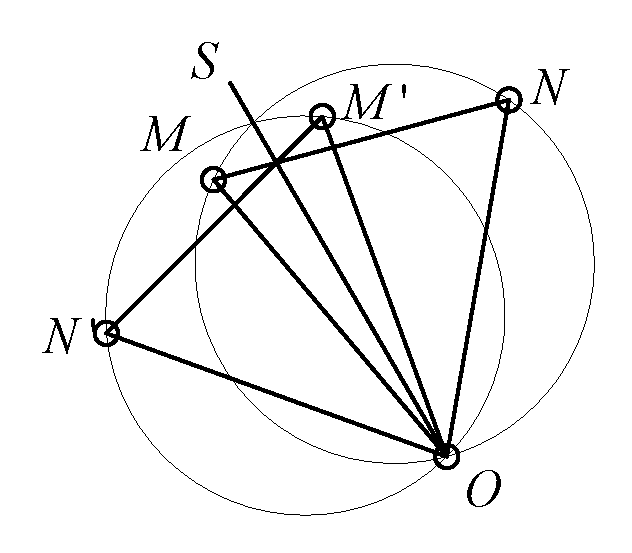
\includegraphics[width = 0.4\textwidth]{图片/幻觉重合.pdf}
    \caption{幻觉的可能位置}
    \label{fig:幻觉重合}
\end{figure}

由已有条件,我们可以得到:$OM=OM'$,$\angle MOS = \angle M'OS$,$\angle NOS = \angle N'OS$。我们可以得到:
\begin{equation}
    \angle MON = \angle M'ON' = \angle MOS + \angle NOS = \angle M'OS + \angle N'OS
\end{equation}
则可以根据,全等三角形的边角边定理,得到$\bigtriangleup MON \cong \bigtriangleup M'ON'$。则可以得到:
\begin{equation}
    \angle N'M'O = \angle NMO
\end{equation}
这样构建起了一个到一一对应关系,对于一个点$M$,我们可以找到一个点$M'$,$\angle N'M'O = \angle NMO$。我们知道,使得$\angle NMO$为固定值的点,在经过$N$和$O$且半径固定的圆上。则使得$\angle N'M'O$为相同固定值的点,在其关于$OS$对称的圆上。

如图所示,这两个圆交与2点,一个是点$O$,另一个点在$OS$上。也就是说,只有点$M$在$OS$上时,才能满足$\angle OMN = \angle OMN'$。

回到各个的问题,想要“幻觉”与真实位置相同,则需要满足$\angle OMN = \angle OMN'$。所以,其必须在$OS$上,如果$N$和$N'$的位置是准确的,那么等价于$M$在极坐标系的极角是与正确位置相同的。

\subsection{额外两架无人机的情况}

接下来,我们讨论有额外两架发射信号的无人机的情况,即除了FY00和FY01外,还有序号分别为$m$和$n$的无人机FY0M和FY0N发射信号,序号为$p$的无人机FY0P接收信号,但是FY0P不知道除了FY00和FY01外的发射信号无人机的序号。序号为$p$的无人机接收到三个角度信息,分别为$\alpha_{0PM}$,$\alpha_{0PN}$和$\alpha_{0P1}$。和上面相同,除了正确位置外,$\alpha_{0PM}$,$\alpha_{0PN}$各会误导出一个错误的位置,我们称之为“幻觉”。只要两个“幻觉”的位置不同,FY0P就可以通过投票的方式得到自己的真实位置。

下面,我们来讨论,两个幻觉的位置在什么时候会重合。

如果,待确定位置无人机的位置的在极坐标系下的极角是正确的,则根据上面的讨论,两个幻觉都和正确位置重合,FY0P可以确定自己的位置。

如果,两个额外发射信号无人机中的任何一架,关于FY0P于与FY01对称,则FY0P可以立即确定自身位置。

我们现在来讨论不同于上面两个特殊情况的一般情况。假设两个“幻觉”重合于真实位置外的任意一点。则如图\ref{fig:两架无人机}所示,图中$D$是FY01位置,$P$是真实位置,$M$和$N$为实际发射信号无人机位置,$M'$和$N'$为被误认为是发射信号无人机位置,$P'$为两个“幻觉重合的位置”。

\begin{figure}[!ht]
    \centering
    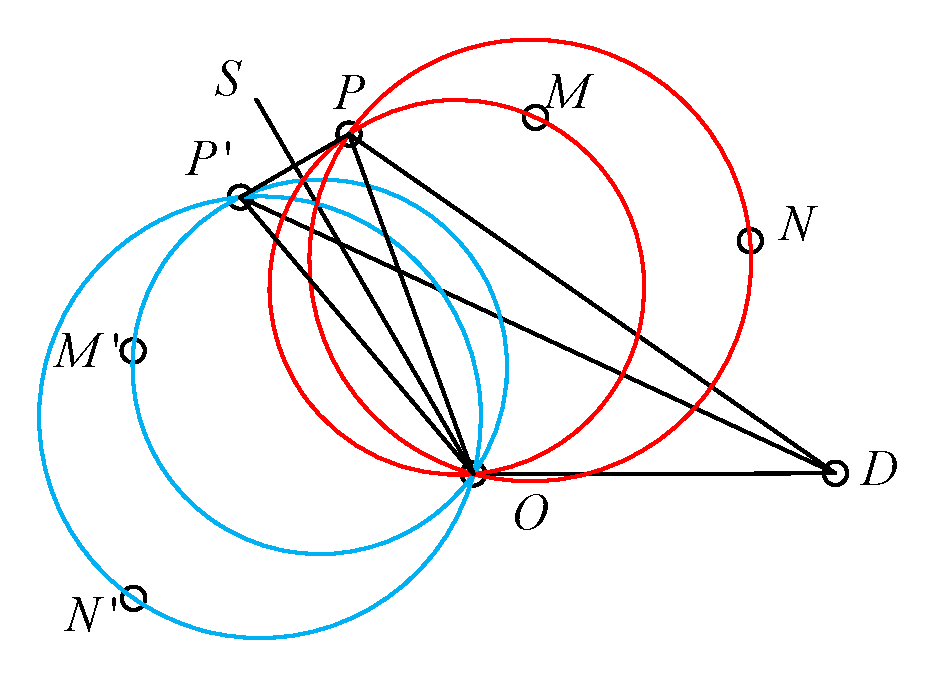
\includegraphics[width = 0.6\textwidth]{图片/两架无人机情况.pdf}
    \caption{两架额外无人机的一般情况}
    \label{fig:两架无人机}
\end{figure}

那么真实位置是红色两个圆的交点,两个“幻觉”重合于蓝色两个圆相交的点。因为两个蓝色的圆是两个红色的圆关于$OS$堆成得到的,则$P$和$P'$也关于$OS$对称。则可以得到
\begin{equation}
    OP = OP'
\end{equation}
因为无论是幻觉还是真实位置还需要满足:
\begin{equation}
    \angle OPD = \angle OP'D
\end{equation}
我们不讨论$P'$和$P$在$OD$两侧的情况,因为这至少要求FY05或FY06的极角偏差$\frac{1}{9}\pi$。那么则$P'$和$P$在$OD$同侧,$O$、$D$、$P$、$P'$四点共圆。无论$D$在哪一侧,我们都可以得到:
\begin{equation}
    \angle PDO + \angle PP'O = \pi
\end{equation}
由于$\bigtriangleup POP'$是等边三角形,$\angle PP'O$是锐角,这要求$\angle PDO$是钝角。若$\angle PDO$不是钝角,则假设不成立,两个“幻觉”不会重合于真实位置以外的点。对于FY02和FY09这两个靠近FY01的无人机来说,这个要求虽然苛刻,但是还是容易达到的。为了研究这一问题,我们以FY09为例,我们设$\Delta\theta$为FY09的极坐标偏差,$\Delta\rho$为FY09的极径偏差,满足以下关系时,$\angle PDO$是锐角:
\begin{equation}
    \frac{\Delta\rho}{r_0} < \frac{1}{\cos\left(\frac{2\pi}{9}-\Delta\theta\right)} - 1
    \label{eq:极径偏差关系}
\end{equation}

我们绘制了FY09在临界状态下,极角偏差与极径偏差的关系图,如图\ref{fig:极坐标偏差关系}中蓝色曲线所示,高于曲线的部分,可能会产生FY0P无法确定自身位置的情况,图中橙色曲线,则为式\ref{eq:误差条件}的要求,高于曲线的部分,FY0P会无法确定发射信号的无人机。我们从图中可以看到,式\ref{eq:误差条件}的要求已经完全覆盖了式\ref{eq:极径偏差关系}的要求,所以不需要引入额外的条件。

\begin{figure}[!ht]
    \centering
    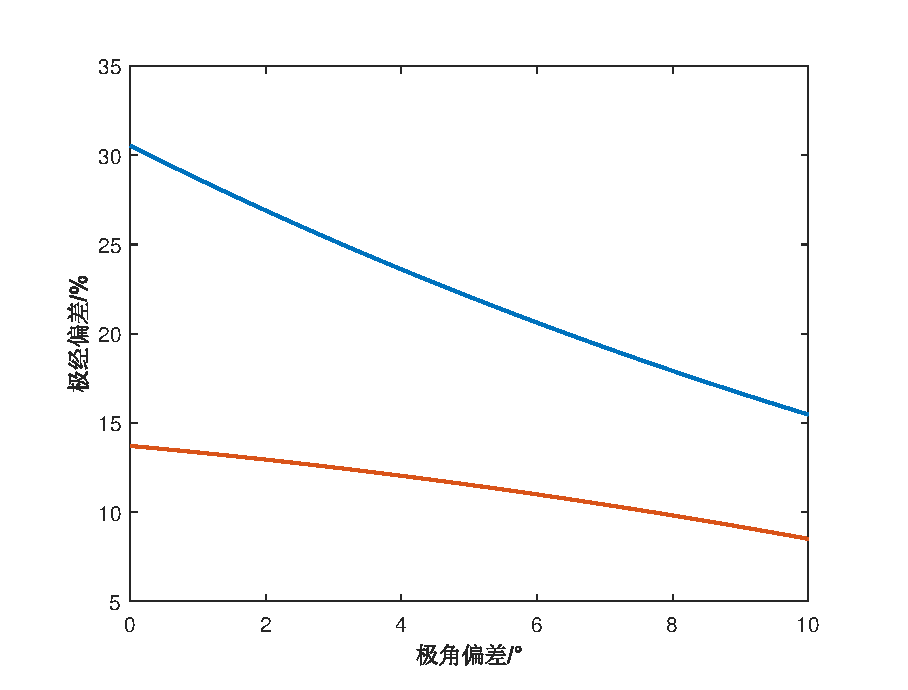
\includegraphics[width = 0.6\textwidth]{图片/极角极径偏差.eps}
    \caption{FY09临界状态下极坐标偏差关系}
    \label{fig:极坐标偏差关系}
\end{figure}

综上所示,对于有额外两架无人机的情况,在无人机位置的偏差满足式\ref{eq:误差条件}时,FY0P都可以通过投票的方式确定自身位置。

%%%%%%%%%%%%%%%%%%%%%%%%%%%%%%%%%%%%%%%%%%%%%%%%%%%%%%%%%%%%%%%%
%                                                              %
%%%%%%%%%%%%%%%%%%%%%%%%%%%%%%%%%%%%%%%%%%%%%%%%%%%%%%%%%%%%%%%%

\section{问题一(3):无人机编队调整}

\subsection{在角度指引下的无人机移动}

对于无人机位置的调整问题,我们首先需要处理的就是,如何根据接收到的角度信息来调整自己的位置。如图\ref{fig:角度指引下无人机调整}所示。$O$为在圆心的发射信号的无人机,$L_1$和$L_2$为在圆周上的两架发射信号的无人机,$R$为需要通过接收的信号调整位置的无人机。在这个例子中,$R$需要从$R_1$的位置移动到$R_2$的位置。
\begin{figure}[!ht]
    \centering
    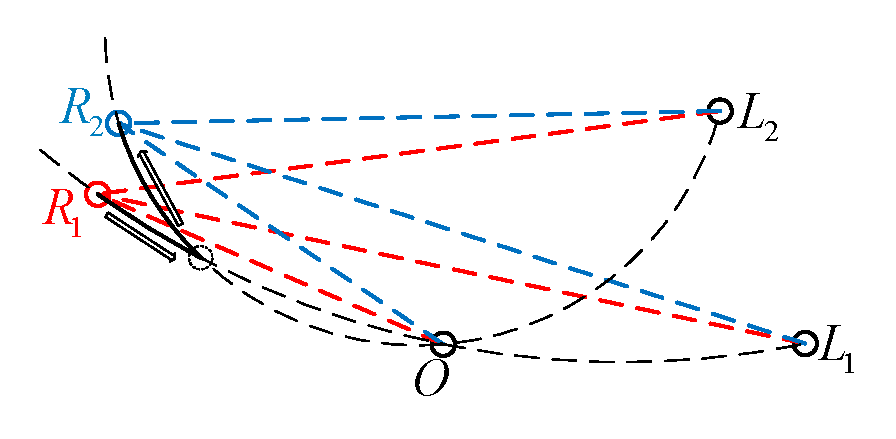
\includegraphics[width=0.6\textwidth]{图片/问题1-3示意图1.pdf}
    \caption{角度指引下无人机调整示意图}
    \label{fig:角度指引下无人机调整}    
\end{figure}

我们给出如下的调整策略:
\begin{enumerate*}
    \item 保持$\angle ORL_1$不变为$\angle OR_1L_1$,顺着梯度方向或梯度下降方向,将$\angle ORL_2$从$\angle OR_1L_2$调整至$\angle OR_2L_2$;
    \item 保持$\angle ORL_2$不变为$\angle OR_2L_2$,顺着梯度方向或梯度下降方向,将$\angle ORL_1$从$\angle OR_1L_1$调整至$\angle OR_2L_1$。
\end{enumerate*}

调整的路线如图\ref{fig:角度指引下无人机调整}中黑色实线和箭头所示。通过这种基于角度指引的无人机移动方案,通过一架位于圆心和两架位于圆周上的无人机发射信号,可以将一架接收信号的无人机在小范围内进行调整,使得其接收到的两个角度信息为指定值。

接下来的无人机编队调整方案中,所有无人机位置的调整都将是基于这种在角度指引下的无人机移动的。

\subsection{无人机编队调整方案}

\subsubsection{调整方案的层次结构}

我们的无人机调整有如下层次结构:
\begin{itemize*}
    \item 针对单架无人机进行单一目的的调整称为“步”;
    \item 所有无人机(除“半径标定机”外)都进行了一“步”调整则称为“轮”。
\end{itemize*}

我们的无人机调整方案共有两种“步”的调整方案:“角度矫正步”、“半径矫正步”。其原则如下:
\begin{itemize*}
    \item 角度矫正步:无人机接收两侧无人机和圆心无人机发出的信号。调整自身位置,使得自身接收到的角度信号为理想角度;
    \item 半径矫正步:无人机接收来关于“半径标定机”对称的无人机、“半径标定机”还有圆心无人机的信号,假设发射信号和接收信号的无人机角度信息是正确的。维持自身、FY00与“半径标定机”形成的夹角不变,调整自身位置,使自身距离FY00的距离与“半径标定机”距离FY00的距离相等。
\end{itemize*}

\subsubsection{角度矫正步}

观察图\ref{fig:角度矫正步},其中,$O$为圆心,$L_1$和$L_2$为在圆周上的两架发射信号的无人机,$R$为圆周上接收信号的无人机,$R'$为我们希望$R$移动到的位置。

\begin{figure}[!ht]
    \centering
    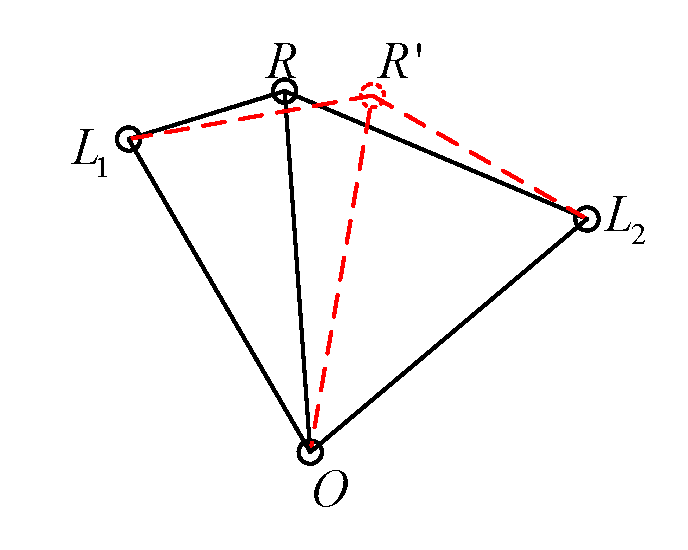
\includegraphics[width=0.5\textwidth]{图片/角度矫正步.pdf}
    \caption{角度矫正步示意图}
    \label{fig:角度矫正步}
\end{figure}

我们知道,在正确位置时,有
\begin{equation}
    \angle R'OL_1 = \frac{2}{9}\pi
\end{equation}
由于$OL_1=OR'$,所以我们可以得到:
\begin{equation}
    \angle R'L_1O = \angle L_1R'O
\end{equation}
则:
\begin{equation}
    \angle R'L_1O = \angle L_1R'O = \frac{\pi - \frac{2}{9}\pi}{2} = \frac{7}{18}\pi
\end{equation}

这样,我们得到了角度矫正步的调整方案:设任意一个无人机FY0N,其顺时针方向的下一个无人机为FY0N-1,逆时针方向的下一个无人机为FY0N+1。FY0N接收到的角度信息为$\alpha_{0NN-1}$和$\alpha_{0NN+1}$,我们需要调整其至$\alpha_{0NN-1}'$和$\alpha_{0NN+1}'$满足如下条件:
\begin{equation}
    \alpha_{0NN-1}' = \alpha_{0NN+1}' = \frac{7}{18}\pi
    \label{eq:角度矫正步}
\end{equation}

\subsubsection{半径矫正步}

图\ref{fig:半径矫正步1}和图\ref{fig:半径矫正步2}展示了半径矫正步的两种不同情况。假设“半径标定机”为FY01,则情况1对应待调整无人机序数为2、3、8和9,情况2对应待调整无人机序数为4、5、6和7。

\begin{figure}[!ht]
    \centering
    \begin{minipage}[t]{0.3\textwidth}
        \centering
        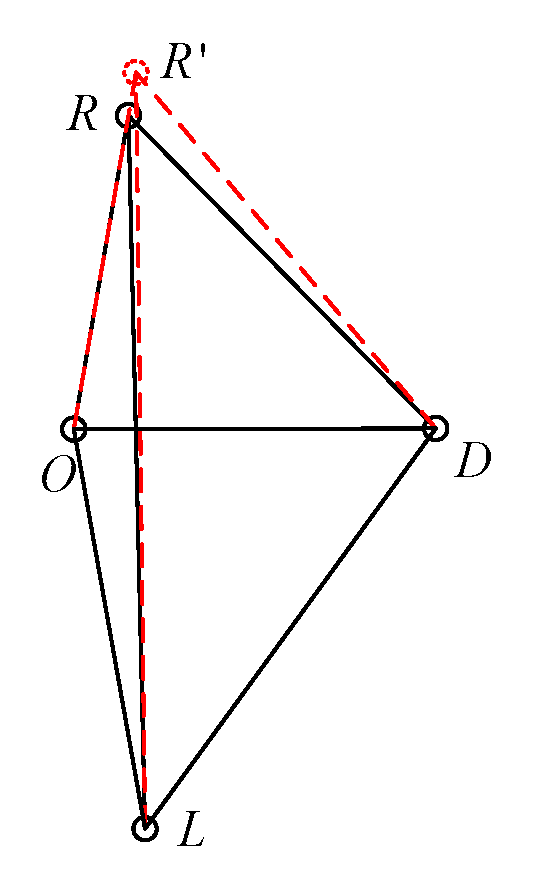
\includegraphics[width=\textwidth]{图片/半径矫正步1.pdf}
        \caption{半径矫正步情况1}
        \label{fig:半径矫正步1}
    \end{minipage}
    \hspace{0.1\textwidth}
    \begin{minipage}[t]{0.45\textwidth}
        \centering
        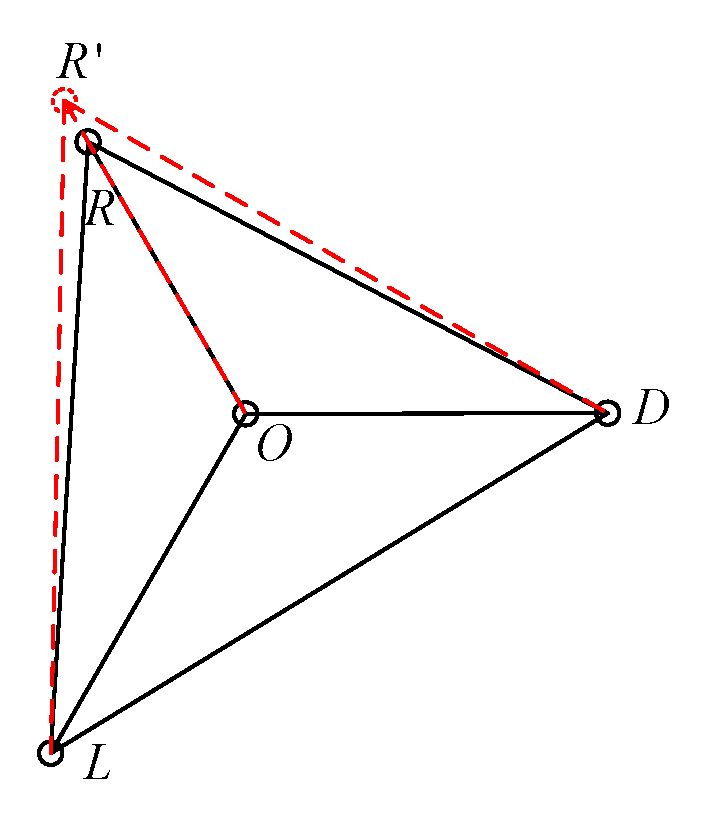
\includegraphics[width=\textwidth]{图片/半径矫正步2.pdf}
        \caption{半径矫正步情况2}
        \label{fig:半径矫正步2}
    \end{minipage}
\end{figure}

我们以情况1为例,我们假设$R$和$L$的角度信息都是对的。如果无人机序数$n$为2或者3,我们可以得到:
\begin{equation}
    \angle LOD = \angle ROD = \frac{2}{9}(n-1)\pi
    \label{eq:上方}
\end{equation}
如果无人机序数$n$为8或者9,我们可以得到:
\begin{equation}
    \angle LOD = \angle ROD = \frac{2}{9}(10-n)\pi
    \label{eq:下方}
\end{equation}
由于$OR'=OD$,所以我们可以得到:
\begin{equation}
    \angle OR'D = \angle ODR' = \frac{\pi - \angle R'OD}{2}
\end{equation}

通过对$\bigtriangleup ORD$使用正弦定理,可以得到:
\begin{equation}
    OR = \frac{OD\,\sin\left(\pi - \angle ROD - \angle ORD\right)}{\sin \angle ORD}
\end{equation}
然后通过对$\bigtriangleup ORL$使用正弦定理,可以得到:
\begin{equation}
    OL = \frac{OR\,\sin{\angle ORL}}{\sin\left(\pi - \angle ROL - \angle ORL\right)}
\end{equation}
其中,$\angle ROL = 2\angle ROD$最后通过对$\bigtriangleup OR'L$使用正弦定理,可以得到方程:
\begin{equation}
    \frac{OR'}{\sin\left(\pi - \angle ROL - \angle OR'L\right)} = \frac{OL}{\sin\angle OR'L}
\end{equation}
整理可以得到:
\begin{equation}
    \frac{\sin\angle ORL\,\sin\left(\angle ROD + \angle ORD\right)\,\sin\left(\angle ROL + \angle OR'L\right)}{\sin\angle ORD\,\sin\left(\angle ROL + \angle ORL\right)\,\sin\angle OR'L} = 1
    \label{eq:初步化简方程}
\end{equation}
我们定义$k$为:
\begin{equation}
    k = \frac{\sin\angle ORL\,\sin\left(\angle ROD + \angle ORD\right)}{\sin\angle ORD\,\sin\left(\angle ROL + \angle ORL\right)}
\end{equation}
则式\ref{eq:初步化简方程}可以变为:
\begin{equation}
    \frac{\sin\left(\angle ROL + \angle OR'L\right)}{\sin\angle OR'L} = \frac{1}{k}
\end{equation}
化简后整理可以得到:
\begin{equation}
    \angle OR'L = \arctan\frac{\sin\angle ROL}{\frac{1}{k}-\cos\angle{ROL}}
\end{equation}

我们依据$\angle OR'L$与$\angle OR'D$的指引,将接收信号的无人机移动到指定位置即可。

情况2的情况基本类似,$\angle ROD$的计算方式当无人机序数为4和5时同式\ref{eq:上方},当计算无人机序数为6和7时同式\ref{eq:下方},唯一的区别在于$\angle ROL = 2\pi - 2\angle ROD$。

这样,我们得到了半径矫正步的调整方案:对于任意一个无人机,通过接收“半径标定机”和其关于“半径标定机”对称的无人机的信号,通过接收的信号,通过上述过程计算出计算出目标角度后,按照目标角度调整自身位置即可。

但是我们发现,该方法在无人机的半径基本正确而角度偏差较大的情况下并不稳定,所以仅作为预处理手段使用。

\subsubsection{调整方案流程}

我们的调整方案流程如下:
\begin{enumerate*}
    \item 首先选择“半径标定机”,其和原点(及FY00)在之后的调整中不会改变位置;
    \item 重复进行迭代矫正。每次重复时,执行一次“角度矫正轮”,除FY00和“半径标定点”外的所有无人机进行依次“角度矫正步”。如果是第一次执行,还会在“角度矫正轮”前,执行一次“半径矫正轮”,除FY00和“半径标定点”外的所有无人机进行依次“半径矫正步”。
\end{enumerate*}

\subsection{调整方案的模拟}

我们在题目给出的信息的基础上,对调整方案进行了模拟。为了衡量无人机组整体位置相对于理想位置的偏差,定义了如下的损失函数:
\begin{equation}
    L = \sum_{i=0}^{9} d_i^2
\end{equation}
其中,$d_i$是序数为$i$的无人机,当前位置与理想位置的欧几里得距离。

我们还模拟了不采取“半径矫正轮”进行预处理的情况,作为对比,来说明“半径矫正轮”的重要性。

无人机在各个阶段的位置如图\ref{fig:无人机位置对比}所示。损失函数随迭代次数的变化如图\ref{fig:损失函数变化}所示。损失函数的具体数值见表\ref{tab:损失函数变化},损失函数1代表不进行半径矫正时的损失函数,损失函数2代表进行半径矫正时的损失函数。

\begin{figure}[!ht]
    \centering
    \begin{minipage}[t]{0.34\textwidth}
        \centering
        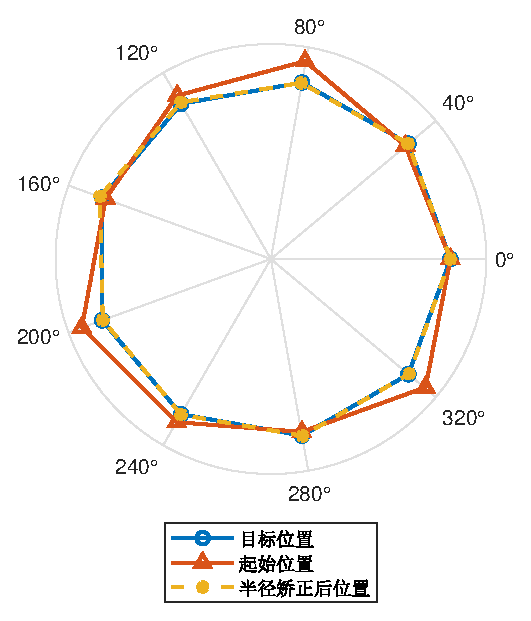
\includegraphics[width=\textwidth]{图片/无人机位置对比.eps}
        \caption{无人机位置对比}
        \label{fig:无人机位置对比}
    \end{minipage}
    \begin{minipage}[t]{0.58\textwidth}
        \centering
        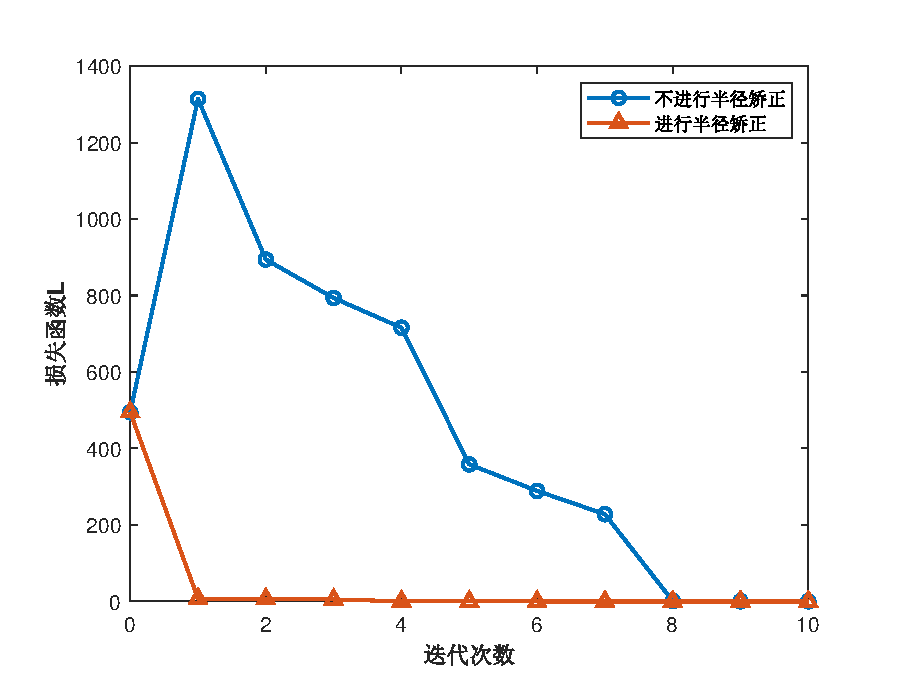
\includegraphics[width=\textwidth]{图片/损失函数变化.eps}
        \caption{损失函数变化情况}
        \label{fig:损失函数变化}
    \end{minipage}
\end{figure}

\begin{table}[!ht]
    \centering
    \caption{损失函数变化情况}
    \label{tab:损失函数变化}
    \begin{tabular}{ccc|ccc}
        \toprule
        迭代次数 & 损失函数1 & 损失函数2 & 迭代次数 & 损失函数1 & 损失函数2 \\ 
        \midrule
        0 & $4.95\times 10^2$ & $4.95\times 10^2$ & 6 & $2.89\times 10^2$ & $4.04\times 10^{-2}$ \\ 
        1 & $1.31\times 10^3$ & $7.41\times 10^0$ & 7 & $2.28\times 10^2$ & $4.26\times 10^{-5}$ \\ 
        2 & $8.94\times 10^2$ & $6.88\times 10^0$ & 8 & $1.17\times 10^0$ & $3.32\times 10^{-8}$ \\ 
        3 & $7.93\times 10^2$ & $5.28\times 10^0$ & 9 & $6.18\times 10^{-1}$ & $1.98\times 10^{-8}$ \\ 
        4 & $7.16\times 10^2$ & $4.01\times 10^{-1}$ & 10 & $3.51\times 10^{-1}$ & $1.23\times 10^{-8}$ \\ 
        5 & $3.59\times 10^2$ & $8.99\times 10^{-2}$ \\ 
        \bottomrule
    \end{tabular}
\end{table}

我们从图中可以看到,“半径矫正轮”可以非常有效地加速模型的收敛。且无论是否增加“半径矫正轮”,无人机都可以通过我们的算法最后逼近正确的位置。

当然,仅凭借1组数据不能说明模型的准确性,我们进行了更多的模拟,这些模拟中的数据为随机产生。我们首先将10个无人机的位置设置在正确位置,然后给除了FY00和FY01外所有的无人机的极坐标角度上加上一个符合$N(0,1)$的偏移,极坐标半径上加上一个符合$N(0,10)$的偏移,这个偏移量远远大于题目中给出的数据的偏移。重新进行了多次模拟,结果如图\ref{fig:多次尝试}所示,我们可以看到,我们的策略工作得是非常稳定的。

\begin{figure}[!ht]
    \centering
    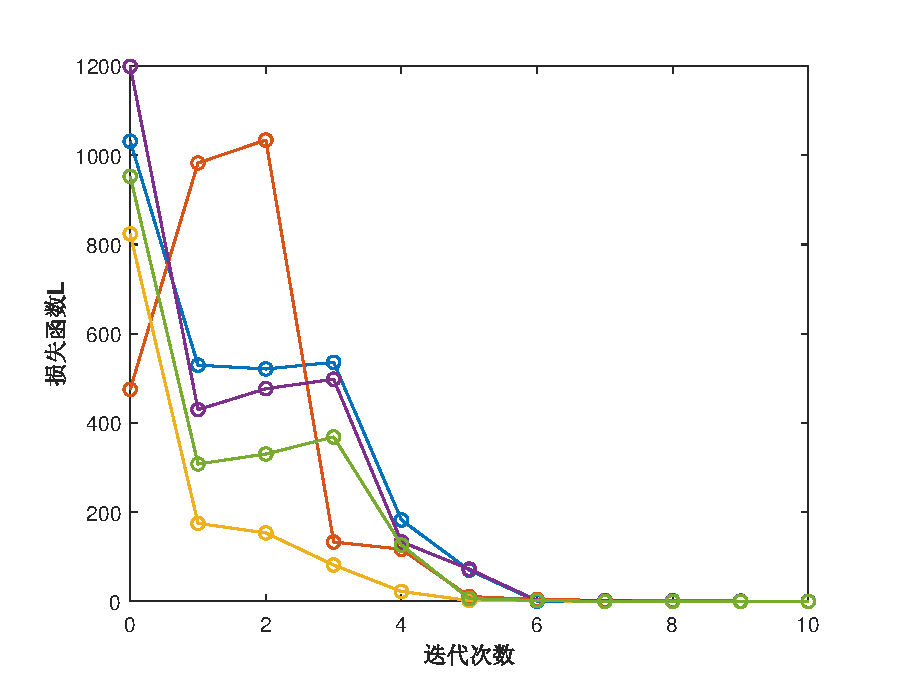
\includegraphics[width=0.6\textwidth]{图片/多次尝试.eps}
    \caption{圆形队列损失函数变化情况}
    \label{fig:多次尝试}
\end{figure}

\subsection{收敛更快的调整策略}

通过上面的讨论,我们已经已经知道了,三个不共线的位置精确的点,通过两个角度信息,可以确定两个点。若给定任意起始点,其可以沿着梯度方向,到达两个点中的一个。我们知道,对于任何队列来说,其中两个点的位置确定了,整个队列的正确位置就确定了。也就是我们需要使用两个无人机标定这个无人机队列。在这个问题中,我们选择了FY00和FY01。所以我们只需要再确定一个位置精确的点,队列中所有的其他点都可以直接通过角度确定。

在这个例子中,我们注意到,FY01、FY04和FY07三等分了圆周,我们可以通过类似的迭代方法,使得FY04和FY07的位置逼近正确位置,然后其他无人机的位置就可以直接通过角度确定。这种方法有一下优点:
\begin{itemize*}
    \item 每次调整都有位置正确的FY01参与,可以加速收敛;
    \item 每次迭代都只有2次调整,可以加快迭代速度。
\end{itemize*}

确定FY01、FY04和FY07位置后,其余无人机可以直接通过与FY04和FY00还有FY07和FY00之间的夹角,直接确定自身位置。我们记一架无人机与FY00和FY04形成的夹角为$\alpha_4$,与FY00和FY07形成的夹角为$\alpha_7$。则其应当调整至的标准角度如表\ref{tab:圆形队列标准角度}所示。

\begin{table}[!ht]
    \centering
    \caption{圆形队列标准角度}
    \label{tab:圆形队列标准角度}
    \begin{tabular}{ccc|ccc}
    \toprule
        无人机编号 & $\alpha_4$ & $\alpha_7$ & 无人机编号 & $\alpha_4$ & $\alpha_7$ \\ 
        \midrule
        FY02 & $\frac{5\pi}{18}$ & $\frac{\pi}{18}$ & FY06 & $\frac{5\pi}{18}$ & $\frac{7\pi}{18}$ \\ 
        FY03 & $\frac{7\pi}{18}$ & $\frac{\pi}{18}$ & FY08 & $\frac{\pi}{18}$ & $\frac{7\pi}{18}$\\ 
        FY05 & $\frac{7\pi}{18}$ & $\frac{5\pi}{18}$ & FY09 & $\frac{\pi}{18}$ & $\frac{5\pi}{18}$ \\ 
    \bottomrule
    \end{tabular}
\end{table}

\subsubsection{4无人机圆周队列调整}

圆周上有3个无人机与圆周上有9个无人机调整方案类似,但有些许不同。我们将FY01重新编号为1,FY04重新编号为2,FY7重新编号为3。

则角度矫正步中理想角度应该改为:
\begin{equation}
    \alpha_{0NN-1}' = \alpha_{0NN+1}' = \frac{2\pi - \frac{2}{3}\pi}{2} = \frac{1}{6}\pi
\end{equation}

半径矫正步中,只会出现情况2,且:
\begin{equation}
    \angle LOD = \angle ROD = \frac{2}{3}\pi
\end{equation}
其余不变。

\subsubsection{调整策略模拟}

我们使用了与图\ref{fig:多次尝试}中相同的起始状态进行模拟。

由于我们的方案是在调整好FY04和FY07位置后,其他无人机立刻移动到正确的位置,并不好展现出迭代中逐渐逼近正确位置的过程。我们修改了我们的模拟方案,在FY04和FY07每次迭代调整结束之后,我们都会立即更新所有无人机的位置,然后计算损失函数。最终我们可以得到图\ref{fig:多次尝试_优化}。

\begin{figure}[!ht]
    \centering
    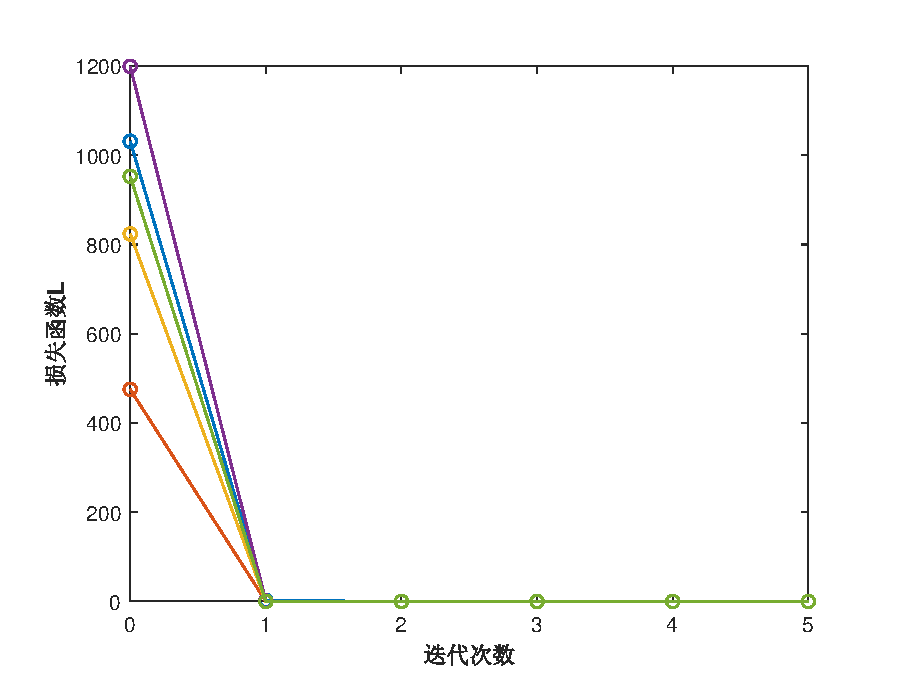
\includegraphics[width=0.6\textwidth]{图片/多次尝试_优化.eps}
    \caption{优化后圆形队列损失函数变化情况}
    \label{fig:多次尝试_优化}
\end{figure}

从中我们可以看出,这种优化后的方法可以非常好得加快收敛速度,可以使得无人机更快地逼近正确位置。

%%%%%%%%%%%%%%%%%%%%%%%%%%%%%%%%%%%%%%%%%%%%%%%%%%%%%%%%%%%%%%%%
%                                                              %
%%%%%%%%%%%%%%%%%%%%%%%%%%%%%%%%%%%%%%%%%%%%%%%%%%%%%%%%%%%%%%%%

\section{问题二:锥形队列调整方案}

\subsection{调整方案}

我们沿用上面的策略,考虑对称性,我们选择FY01和FY05的位置来标定无人队列。接下来,我们还需要确定一个位置固定的点。观察图\ref{fig:问题2示意图},我们可以发现,在位置正确的情况下,FY01、FY07和FY10在以FY05为圆心的圆周上,且将圆周三等分。
\begin{figure}[!ht]
    \centering
    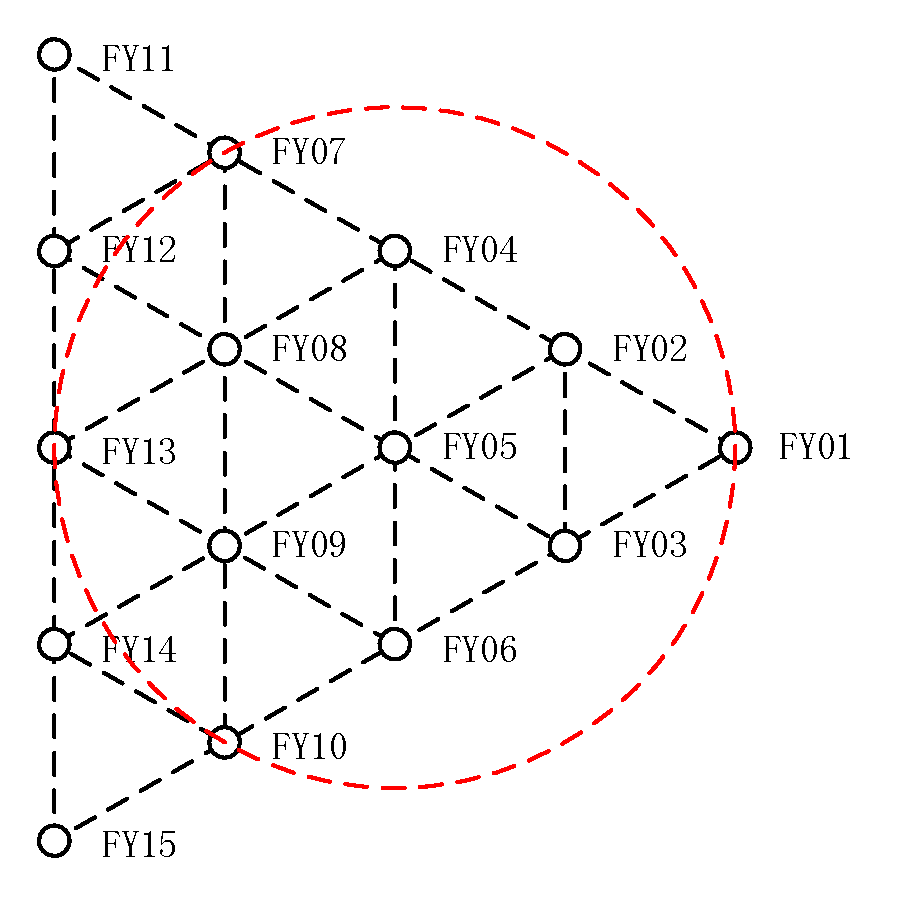
\includegraphics[width=0.5\textwidth]{图片/问题2示意图.pdf}
    \caption{问题2示意图}
    \label{fig:问题2示意图}
\end{figure}

这样,我们就可以给出我们的调整策略:

\begin{enumerate*}
    \item 按照问题一中的策略,将FY01、FY05、FY07和FY10看作一个圆形无人机编队。将FY05作为圆心,FY01作为“半径标定机”。调整FY05和FY07的位置,使其逼近正确位置;
    \item FY05和FY07的位置正确后,其他无人机直接通过与FY07和FY05还有FY10和FY05之间的夹角,直接确定自身位置。
\end{enumerate*}

我们记一架无人机与FY05和FY07形成的夹角为$\alpha_7$,与FY05和FY10形成的夹角为$\alpha_{10}$。则其应当调整至的标准角度如表\ref{tab:锥形队列标准角度}所示。

\begin{table}[!ht]
    \centering
    \caption{15架无人机队列标准角度}
    \label{tab:锥形队列标准角度}
    \begin{tabular}{ccc|ccc}
    \toprule
        无人机编号 & $\alpha_7$ & $\alpha_{10}$ & 无人机编号 & $\alpha_7$ & $\alpha_{10}$ \\ 
        \midrule
        FY02 & $\frac{\pi}{3}$ & $\arctan\frac{\sqrt{3}}{5}$ & FY11 & $\arctan\frac{\sqrt{3}}{5}$ & $\arctan\frac{5\sqrt{3}}{17}$ \\ 
        FY03 & $\arctan\frac{\sqrt{3}}{5}$ & $\frac{\pi}{3}$ & FY12 & $\frac{\pi}{3}$ & $\arctan\frac{\sqrt{3}}{2}$\\ 
        FY04 & $\frac{2\pi}{3}$ & $\arctan\frac{\sqrt{3}}{5}$ & FY13 & $\frac{\pi}{3}$ & $\frac{\pi}{3}$ \\ 
        FY06 & $\arctan\frac{\sqrt{3}}{5}$ & $\frac{2\pi}{3}$ & FY14 & $\arctan\frac{\sqrt{3}}{2}$ & $\frac{\pi}{3}$ \\ 
        FY08 & $\frac{2\pi}{3}$ & $\frac{\pi}{3}$ & FY15 & $\arctan\frac{5\sqrt{3}}{17}$ & $\arctan\frac{\sqrt{3}}{5}$ \\ 
        FY09 & $\frac{\pi}{3}$ & $\frac{2\pi}{3}$ \\ 
    \bottomrule
    \end{tabular}
\end{table}

\subsection{调整方案的模拟}

我们首先将15个无人机的位置设置在正确位置,然后给除了FY01和FY05外所有的无人机加上一个长度随机,方向随机的偏移。这个偏移的长度符合$U\left(0,\frac{S}{2}\right)$,其中$S$为等边三角形的边长。然后我们使用我们的调整方案,将无人机移动到正确的位置。

同样的,我们修改了我们的模拟方案,在FY07和FY10每次迭代调整结束之后,我们都会立即更新所有无人机的位置,然后计算损失函数:
\begin{equation}
    L = \sum_{i=1}^{15} d_i^2
\end{equation}

最终,调整前后的无人机位置对比如图\ref{fig:无人机位置对比_锥形}所示,损失函数随迭代次数的变化如图\ref{fig:损失函数变化_锥形}所示。损失函数的具体数值见表\ref{tab:损失函数变化_锥形}。

\begin{figure}[!ht]
    \centering
    \begin{minipage}[t]{0.43\textwidth}
        \centering
        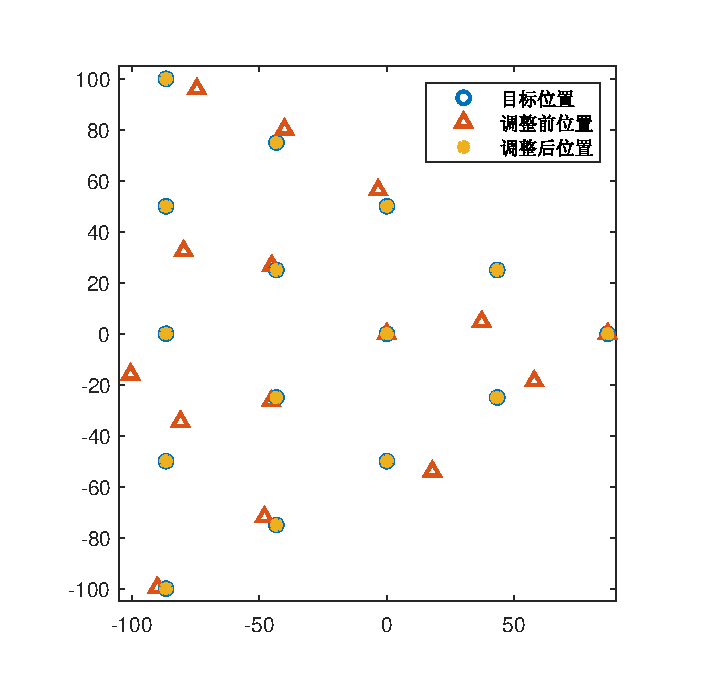
\includegraphics[width=\textwidth]{图片/无人机位置对比_锥形.eps}
        \caption{锥形队列无人机位置对比}
        \label{fig:无人机位置对比_锥形}
    \end{minipage}
    \begin{minipage}[t]{0.56\textwidth}
        \centering
        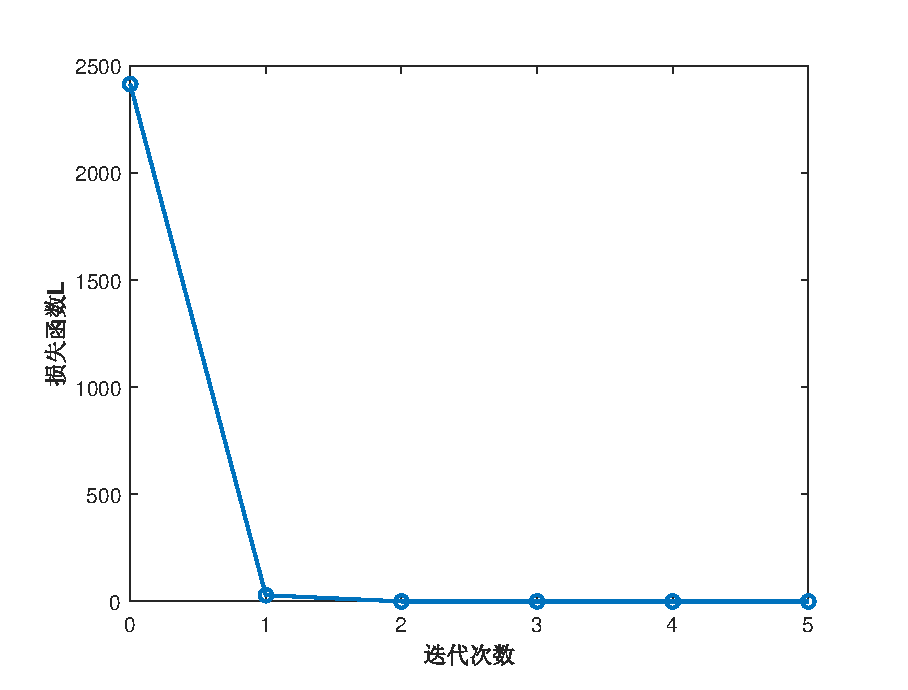
\includegraphics[width=\textwidth]{图片/损失函数变化_锥形.eps}
        \caption{锥形队列损失函数变化情况}
        \label{fig:损失函数变化_锥形}
    \end{minipage}
\end{figure}

\begin{table}[!ht]
    \centering
    \caption{锥形队列损失函数变化情况}
    \label{tab:损失函数变化_锥形}
    \begin{tabular}{cc|cc}
        \toprule
        迭代次数 & 损失函数 & 迭代次数 & 损失函数 \\
        \midrule
        0 & $2.41\times 10^3$ & 3 & $3.70\times 10^{-10}$ \\ 
        1 & $2.91\times 10^1$ & 4 & $3.70\times 10^{-10}$ \\ 
        2 & $3.70\times 10^{-10}$ & 5 & $3.70\times 10^{-10}$ \\ 
        \bottomrule
    \end{tabular}
\end{table}

我们从中可以看出,我们的对于锥形队列无人机的调整方案也非常有效,可以很好地将无人机固定在正确的位置。

%%%%%%%%%%%%%%%%%%%%%%%%%%%%%%%%%%%%%%%%%%%%%%%%%%%%%%%%%%%%%%%%
%                                                              %
%%%%%%%%%%%%%%%%%%%%%%%%%%%%%%%%%%%%%%%%%%%%%%%%%%%%%%%%%%%%%%%%

\section{模型评价}

我们的模型具有以下优点:
\begin{itemize*}
    \item 在第一问第1小问中,我们的基于两圆相交的定位模型,可以给出待定位无人机位置的解析解;
    \item 在第一问第2小问中,我们基于严格的数学证明,证明了在待定无人机的位置偏差满足式\ref{eq:误差条件}的情况下,通过额外两架无人机发射的信号,就可以确定待定无人机的位置;
    \item 在第一问第2小问中,我们还讨论了一架额外无人机就可以确定待定无人机位置的情况;
    \item 在第一问第3小问中,我们提出了一种基于迭代的调整方案,可以使得无人机队列快速逼近正确位置,并且给出了收敛更快的优化后的调整策略;
    \item 在第二问中,我们将其转化为了与第一问相似的问题,并进行了解决。
\end{itemize*}

但是我们的模型还具有以下不足:
\begin{itemize*}
    \item 我们的模型对于误差范围更加极端的情况,适应性较差;
    \item 对于第二问,没有讨论待定无人机位置偏差不满足式\ref{eq:误差条件}的情况。
\end{itemize*}

%%%%%%%%%%%%%%%%%%%%%%%%%%%%%%%%%%%%%%%%%%%%%%%%%%%%%%%%%%%%%%%%
%                                                              %
%%%%%%%%%%%%%%%%%%%%%%%%%%%%%%%%%%%%%%%%%%%%%%%%%%%%%%%%%%%%%%%%

\section{模型改进与推广}

我们可以考虑如下的改进思路:
\begin{itemize*}
    \item 可以考虑无人机之间可以互相通信的情况;
    \item 可以考虑无人机按非中心对称的方式排列的情况;
    \item 可以考虑三维情况下的无人机定位问题;
\end{itemize*}

而且我们的模型实际上并没有使用无人机所特有的性质,其可以推广到所有需要进行二维平面无源定位的情况。

%%%%%%%%%%%%%%%%%%%%%%%%%%%%%%%%%%%%%%%%%%%%%%%%%%%%%%%%%%%%%%%%
%%%%%%%%%%%%%%%%%%%%%%%%%%%%%%%%%%%%%%%%%%%%%%%%%%%%%%%%%%%%%%%%
%                            参考文献                           %
%%%%%%%%%%%%%%%%%%%%%%%%%%%%%%%%%%%%%%%%%%%%%%%%%%%%%%%%%%%%%%%%
%%%%%%%%%%%%%%%%%%%%%%%%%%%%%%%%%%%%%%%%%%%%%%%%%%%%%%%%%%%%%%%%

\nocite{sxjm}

\bibliographystyle{gbt7714-numerical}
\bibliography{sample}

%%%%%%%%%%%%%%%%%%%%%%%%%%%%%%%%%%%%%%%%%%%%%%%%%%%%%%%%%%%%%%%%
%%%%%%%%%%%%%%%%%%%%%%%%%%%%%%%%%%%%%%%%%%%%%%%%%%%%%%%%%%%%%%%%
%                             附录                             %
%%%%%%%%%%%%%%%%%%%%%%%%%%%%%%%%%%%%%%%%%%%%%%%%%%%%%%%%%%%%%%%%
%%%%%%%%%%%%%%%%%%%%%%%%%%%%%%%%%%%%%%%%%%%%%%%%%%%%%%%%%%%%%%%%

\newpage
\appendix
\centerline{\Large\heiti\textbf{附录}}

\section{使用代码}

\subsection{calculateAngle.m}
\begin{minted}[breaklines]{matlab}
function angle = calculateAngle(N1,N2,O)
%CALCULATEANGLE 计算角N1ON2
%   其中O为角的顶点,N1、N2和O用二维行向量表示笛卡尔坐标系下的坐标
%   返回角度的单位为弧度
ON1 = N1 - O;
ON2 = N2 - O;
angle = atan2( ...
    norm(cross([ON1,0],[ON2,0])), ...
    dot(ON1,ON2) ...
    );
end
\end{minted}

\subsection{moveToCertainAngle.m}
\begin{minted}[breaklines]{matlab}
function newR = moveToCertainAngle(A,B,O,R,ARO,BRO)
%MOVETOCERTAINANGLE 将R移动到newR位置,使得角ARO与角BRO为特定值
%   A,B,O,R为用二维行向量表示笛卡尔坐标系下的坐标
%   ARO与BRO为指定角度,弧度制
fun = @(x)[calculateAngle(A,O,x)-ARO,calculateAngle(B,O,x)-BRO];
opt = optimset('Display','off','FunValCheck','on','TolFun',1e-9);
newR = fsolve(fun,R,opt);
end
\end{minted}

\subsection{radiusAdjust.m}
\begin{minted}[breaklines]{matlab}
function points = radiusAdjust(points,Rid,Did,O)
%RADIUSADJUST 对points中Rid的无人机以Did为标定进行半径调整

intervel = mod(Rid - Did, length(points));
Lid = Did - intervel;
while Lid < 1 || Lid > length(points)
    if(Lid < 1)
        Lid = Lid + length(points);
    else
        Lid = Lid - length(points);
    end
end

ROD = intervel*2*pi/length(points);
if ROD > pi
    ROD = 2*pi-ROD;
end

ROL = ROD*2;
if ROL > pi
    ROL = 2*pi-ROL;
end

OR1D = (pi - ROD) ./ 2;
ORD = calculateAngle(points(Did,:),O,points(Rid,:));
ORL = calculateAngle(points(Lid,:),O,points(Rid,:));

k = sin(ORL) * sin(ROD + ORD) / (sin(ORD) * sin(ROL + ORL));
OR1L = atan(sin(ROL)./(1./k - cos(ROL)));

points(Rid,:) = moveToCertainAngle(points(Did,:), points(Lid,:), O, points(Rid,:), OR1D, OR1L);

end
\end{minted}

\subsection{angleAdjust.m}
\begin{minted}[breaklines]{matlab}
function points = angleAdjust(points,id,O)
%ANGLEADJUST 对Points中指定的id的点进行角度矫正

% 顺时针方向下一个点
if id == length(points)
    left = 1;
else
    left = id + 1;
end
% 顺时针方向上一个点
if id == 1
    right = length(points);
else
    right = id - 1;
end

target = (pi - 2*pi / length(points)) / 2;

points(id,:) = moveToCertainAngle(points(left,:), points(right,:), O, points(id,:), target, target);

end
\end{minted}

\subsection{question1\_3.m}
\begin{minted}[breaklines]{matlab}
clearvars

% 初始化
FY00pc = [0,0]; FY00xy = [0,0];
FYpc_g = [100,0;98,40.10;112,80.21;105,119.75;98,159.86;
    112,199.96;105,240.07;98,280.17;112,320.28];
FYpc_t = [100,0;100,40;100,80;100,120;100,160;100,200;
    100,240;100,280;100,320];
FYxy_t = zeros(9,2);FYxy_g = zeros(9,2);FYxy = zeros(9,2);
[FYxy_g(:,1),FYxy_g(:,2)] = pol2cart(deg2rad(FYpc_g(:,2)),FYpc_g(:,1));
[FYxy_t(:,1),FYxy_t(:,2)] = pol2cart(deg2rad(FYpc_t(:,2)),FYpc_t(:,1));

times = 10;

% 进行半径矫正组
[FYxy(:,1),FYxy(:,2)] = pol2cart(deg2rad(FYpc_g(:,2)),FYpc_g(:,1));
L1 = zeros(1,times + 1);
L1(1) = sum((FYxy(:,1) - FYxy_t(:,1)).^2 + (FYxy(:,2) - FYxy_t(:,2)).^2);
for k = 1:times
    if k == 1
        for i = 2:9
            FYxy = radiusAdjust(FYxy,i,1,FY00xy);
        end
        [tempTheta, tempRho] = cart2pol(FYxy(:,1),FYxy(:,2));
    end
    for i = 2:9
        FYxy = angleAdjust(FYxy,i,FY00xy);
    end
    L1(1 + k) = sum((FYxy(:,1) - FYxy_t(:,1)).^2 + (FYxy(:,2) - FYxy_t(:,2)).^2);
end

% 不进行半径矫正组
[FYxy(:,1),FYxy(:,2)] = pol2cart(deg2rad(FYpc_g(:,2)),FYpc_g(:,1));
L2 = zeros(1,times + 1);
L2(1) = sum((FYxy(:,1) - FYxy_t(:,1)).^2 + (FYxy(:,2) - FYxy_t(:,2)).^2);
for k = 1:times
    for i = 2:9
        FYxy = angleAdjust(FYxy,i,FY00xy);
    end
    L2(1 + k) = sum((FYxy(:,1) - FYxy_t(:,1)).^2 + (FYxy(:,2) - FYxy_t(:,2)).^2);
end

f1 = figure(1);
polarplot(deg2rad(FYpc_t([1:end,1],2)), FYpc_t([1:end,1],1), '-o', LineWidth=1.5)
hold on
polarplot(deg2rad(FYpc_g([1:end,1],2)), FYpc_g([1:end,1],1), '-^', LineWidth=1.5)
polarplot(tempTheta([1:end,1]), tempRho([1:end,1]),'--*', LineWidth=1.5)
legend("目标位置", "起始位置", "半径矫正后位置", Location="southoutside")
rticks([])
thetaticks([0 40 80 120 160 200 240 280 320])

f2 = figure(2);
plot(0:1:times,L2,'-o',LineWidth=1.5)
hold on
plot(0:1:times,L1,'-^',LineWidth=1.5)
xlabel("迭代次数")
ylabel("损失函数L")
legend(["不进行半径矫正","进行半径矫正"])
\end{minted}

\subsection{question1\_3\_2.m}
\begin{minted}[breaklines]{matlab}
clearvars

% 初始化
FY00pc = [0,0]; FY00xy = [0,0];
FYpc_t = [100,0;100,40;100,80;100,120;100,160;100,200;
    100,240;100,280;100,320];
FYxy_t = zeros(9,2);
[FYxy_t(:,1),FYxy_t(:,2)] = pol2cart(deg2rad(FYpc_t(:,2)),FYpc_t(:,1));

times = 10;
num = 5;
L = zeros(num,times + 1);

rng(20240418)

% 进行半径矫正组
for j = 1:num
    FYpc_g = FYpc_t;
    FYpc_g(2:end,2) = FYpc_g(2:end,2) + normrnd(0,1,[8,1]);
    FYpc_g(2:end,1) = FYpc_g(2:end,1) + normrnd(0,10,[8,1]);
    FYxy = zeros(9,2);
    [FYxy(:,1),FYxy(:,2)] = pol2cart(deg2rad(FYpc_g(:,2)),FYpc_g(:,1));
    L(j,1) = sum((FYxy(:,1) - FYxy_t(:,1)).^2 + (FYxy(:,2) - FYxy_t(:,2)).^2);
    for k = 1:times
        if k == 1
            for i = 2:9
                FYxy = radiusAdjust(FYxy,i,1,FY00xy);
            end
            [tempTheta, tempRho] = cart2pol(FYxy(:,1),FYxy(:,2));
        end
        for i = 2:9
            FYxy = angleAdjust(FYxy,i,FY00xy);
        end
        L(j,1 + k) = sum((FYxy(:,1) - FYxy_t(:,1)).^2 + (FYxy(:,2) - FYxy_t(:,2)).^2);
    end
end

f = figure(1);
for i = 1:num
    plot(0:1:times,L(i,1:end),'-o',LineWidth=1)
    hold on
end
xlabel("迭代次数")
ylabel("损失函数L")
\end{minted}

\subsection{question1\_3\_3.m}
\begin{minted}[breaklines]{matlab}
clearvars

% 初始化
FY00pc = [0,0]; FY00xy = [0,0];
FYpc_t = [100,0;100,40;100,80;100,120;100,160;100,200;
    100,240;100,280;100,320];
FYxy_t = zeros(9,2);
[FYxy_t(:,1),FYxy_t(:,2)] = pol2cart(deg2rad(FYpc_t(:,2)),FYpc_t(:,1));

times = 5;
num = 5;
L = zeros(num,times + 1);

rng(20240418)

for j = 1:num
    FYpc_g = FYpc_t;
    FYpc_g(2:end,2) = FYpc_g(2:end,2) + normrnd(0,1,[8,1]);
    FYpc_g(2:end,1) = FYpc_g(2:end,1) + normrnd(0,10,[8,1]);
    FYxy = zeros(9,2);
    [FYxy(:,1),FYxy(:,2)] = pol2cart(deg2rad(FYpc_g(:,2)),FYpc_g(:,1));
    L(j,1) = sum((FYxy(:,1) - FYxy_t(:,1)).^2 + (FYxy(:,2) - FYxy_t(:,2)).^2);
    for k = 1:times
        c147 = FYxy([1,4,7],:);
        if k == 1
            for i = 2:3
                c147 = radiusAdjust(c147,i,1,FY00xy);
            end
        end
        for i = 2:3
            c147 = angleAdjust(c147,i,FY00xy);
        end
        FYxy([1,4,7],:) = c147;
        % 调整无人机所用函数
        fmid = @(x) moveToCertainAngle( ...
            FYxy(4,:),FYxy(7,:),FY00xy,FYxy(x,:), ...
            calculateAngle(FYxy_t(4,:),FY00xy,FYxy_t(x,:)), ...
            calculateAngle(FYxy_t(7,:),FY00xy,FYxy_t(x,:)));
        % 依次根据角度调整剩下的无人机
        FYxy(2,:) = fmid(2);
        FYxy(3,:) = fmid(3);
        FYxy(5,:) = fmid(5);
        FYxy(6,:) = fmid(6);
        FYxy(8,:) = fmid(8);
        FYxy(9,:) = fmid(9);
        L(j,1 + k) = sum((FYxy(:,1) - FYxy_t(:,1)).^2 + (FYxy(:,2) - FYxy_t(:,2)).^2);
    end
end

f = figure(1);
for i = 1:num
    plot(0:1:times,L(i,1:end),'-o',LineWidth=1)
    hold on
end
xlabel("迭代次数")
ylabel("损失函数L")
\end{minted}

\subsection{question2.m}
\begin{minted}[breaklines]{matlab}
clearvars

sideLength = 50;    % 等边三角形边长
times = 5;
% 标准位置
FYxy_t = [sqrt(3),0;sqrt(3)/2,1/2;sqrt(3)/2,-1/2;0,1;0,0;
    0,-1;-sqrt(3)/2,3/2;-sqrt(3)/2,1/2;-sqrt(3)/2,-1/2;-sqrt(3)/2,-3/2;
    -sqrt(3),2;-sqrt(3),1;-sqrt(3),0;-sqrt(3),-1;-sqrt(3),-2] * sideLength;
% 初始位置,在标准位置上添加偏差,FY01和FY05作为基准,保持不变
FYxy_g = FYxy_t;
rng(20240415)   %指定随机数种子,保证可重复性
for i = 1:15
    if i == 1 || i==5
        continue
    end
    eRho = unifrnd(0,sideLength/2);
    eTheta = unifrnd(0,2*pi);
    FYxy_g(i,1) = FYxy_g(i,1) + eRho * cos(eTheta);
    FYxy_g(i,2) = FYxy_g(i,2) + eRho * sin(eTheta);
end
FYxy = FYxy_g;

% 调整FY01,FY07和FY10使其在以FY05为圆心的圆上
c1710 = FYxy([1,7,10],:);
L = zeros(1,times + 1);
L(1) = sum((FYxy(:,1) - FYxy_t(:,1)).^2 + (FYxy(:,2) - FYxy_t(:,2)).^2);
for k = 1:times
    if k == 1
        for i = 2:3
            c1710 = radiusAdjust(c1710,i,1,FYxy(5,:));
        end
    end
    for i = 2:3
        c1710 = angleAdjust(c1710,i,FYxy(5,:));
    end
    FYxy([1,7,10],:) = c1710;
    % 调整无人机所用函数
    fmid = @(x) moveToCertainAngle( ...
        FYxy(7,:),FYxy(10,:),FYxy(5,:),FYxy(x,:), ...
        calculateAngle(FYxy_t(7,:),FYxy_t(5,:),FYxy_t(x,:)), ...
        calculateAngle(FYxy_t(10,:),FYxy_t(5,:),FYxy_t(x,:)));
    % 依次根据角度调整剩下的无人机
    FYxy(2,:) = fmid(2);
    FYxy(3,:) = fmid(3);
    FYxy(4,:) = fmid(4);
    FYxy(6,:) = fmid(6);
    FYxy(8,:) = fmid(8);
    FYxy(9,:) = fmid(9);
    FYxy(11,:) = fmid(11);
    FYxy(12,:) = fmid(12);
    FYxy(13,:) = fmid(13);
    FYxy(14,:) = fmid(14);
    FYxy(15,:) = fmid(15);
    L(1 + k) = sum((FYxy(:,1) - FYxy_t(:,1)).^2 + (FYxy(:,2) - FYxy_t(:,2)).^2);
end

f1 = figure(1);
plot(FYxy_t(:,1),FYxy_t(:,2),'o',LineWidth=1.5)
hold on
plot(FYxy_g(:,1),FYxy_g(:,2),'^',LineWidth=1.5)
plot(FYxy(:,1),FYxy(:,2),'*',LineWidth=1.5)
axis equal
axis([-105,90,-105,105])
legend(["目标位置","调整前位置","调整后位置"])

f2 = figure(2);
plot(0:1:times,L,'-o',LineWidth=1.5)
xlabel("迭代次数")
ylabel("损失函数L")
\end{minted}


\end{document}